%% This is a sample manuscript marked up using the
%% AASTeX v5.x LaTeX 2e macros.

%% The first piece of markup in an AASTeX v5.x document
%% is the \documentclass command. LaTeX will ignore
%% any data that comes before this command.

%% The command below calls the preprint style
%% which will produce a one-column, single-spaced document.
%% Examples of commands for other substyles follow. Use
%% whichever is most appropriate for your purposes.
%%

%\documentclass[11pt,preprint2]{aastex}
% manuscript produces a one-column, double-spaced document:
%\documentclass[manuscript]{aastex}
%% preprint2 produces a double-column, single-spaced document:

%\documentclass{emulateapj}
\documentclass[preprint]{aastex}

\usepackage{natbib}
\usepackage{amsmath}
\bibliographystyle{apj}
\usepackage{graphicx}

%% Sometimes a paper's abstract is too long to fit on the
%% title page in preprint2 mode. When that is the case,
%% use the longabstract style option.

%% \documentclass[preprint2,longabstract]{aastex}

%% If you want to create your own macros, you can do so
%% using \newcommand. Your macros should appear before
%% the \begin{document} command.
%%
%% If you are submitting to a journal that translates manuscripts
%% into SGML, you need to follow certain guidelines when preparing
%% your macros. See the AASTeX v5.x Author Guide
%% for information.

%% You can insert a short comment on the title page using the command below.

%\slugcomment{Not to appear in Nonlearned J., 45.}

%% If you wish, you may supply running head information, although
%% this information may be modified by the editorial offices.
%% The left head contains a list of authors,
%% usually a maximum of three (otherwise use et al.).  The right
%% head is a modified title of up to roughly 44 characters.
%% Running heads will not print in the manuscript style.

%\shorttitle{HERA Dish Beam Measurements Memo, Rev $\alpha$}
%\shortauthors{Neben}

%% This is the end of the preamble.  Indicate the beginning of the
%% paper itself with \begin{document}.

\begin{document}

\title{HERA Dish Beam Measurements Memo}

%% Use \author, \affil, and the \and command to format
%% author and affiliation information.
%% Note that \email has replaced the old \authoremail command
%% from AASTeX v4.0. You can use \email to mark an email address
%% anywhere in the paper, not just in the front matter.
%% As in the title, use \\ to force line breaks.

\author{Abraham Neben, Rich Bradley, Jackie Hewitt, others}
%\affil{MIT Kavli Institute, Massachusetts Institute of Technology, Cambridge, MA, 02139 USA}

\author{Oct 26, 2015}

%% Notice that each of these authors has alternate affiliations, which
%% are identified by the \altaffilmark after each name.  Specify alternate
%% affiliation information with \altaffiltext, with one command per each
%% affiliation.

%% Mark off your abstract in the ``abstract'' environment. In the manuscript
%% style, abstract will output a Received/Accepted line after the
%% title and affiliation information. No date will appear since the author
%% does not have this information. The dates will be filled in by the
%% editorial office after submission.

\begin{abstract}
We deploy the 137\,MHz ORBCOMM beam mapping system of \citet{neben15} at the site of the HERA prototype at NRAO--Green Bank. This technique measures the beam of an antenna-under-test relative to that of a well-modeled reference antenna. We characterize environmental systematics such as reflections and multipath effects by comparing the measured beams of different reference antennas, then measure the beam pattern of the east-most HERA dish as a function of feed height over the dish surface. With the feed at the nominal focus of 4.5\,m over the dish surface, the collecting area is observed to be 68.5\,m$^2$, agreeing with simulations. We also simulate delay spectra on baselines of different lengths and orientations at different LSTs for measured and model beams, and quantify the severity of and uncertainties in the delay space horizon brightening termed the ``pitchfork effect'' by \citet{nithya15}. Future measurements will study the dish beam in the presence of adjacent dishes, quantifying levels of cross-talk and cross-coupling.
\end{abstract}

%\keywords{instrumentation: interferometers --- techniques: interferometric --- cosmology: observations --- dark ages, reionization, first stars}


%\section{Introduction}

%must use frequency structure to separate FGs from signal
%a certain amount of freq structure is imprinted onto smooth sources due to the frequency-dependent sampling function of an interferometer
%also by faraday rotation and the bandpass (citations)

%leakage is due to bandpass, frequency flagging, finite bandwidth. can be mitigated by subtraction in the delay spectrum (CLEAN), giving up on wedge modes, or subtraction in image space with foreground modeling, likely will have to give up on wedge modes too unless have incredible calibration and imaging fidelity, as LOFAR is attempting. Large risk of signal loss and calibration-induced transfer of spectral structure from long baselines to short ones

%hera is pursuing two relatively orthogonal power spectrum analyses (imaging and delay transform)

%the other papers in this series quantify the degree of spectral structure induced by the dish bandpass in measurement and modeling, we focus in this section on foreground leakage due to the finite bandwidth as a function of the beam response at different delays in the sky. Nithya discuss this is detail nithya15,nithya15b

%\citet{nithya15,nithya15b} 
%for a power spectrum analysis, note that these tests test how leakage varies as a function of the brightness of emission at different delays, not leakage due to beam frequency dependence (ie, either pattern or overall gain)

\section{ORBCOMM Beam Mapping System Review}

We briefly review the beam mapping system detailed by \citet{neben15}, then discuss application of system to the prototype HERA array at NRAO--Green Bank. The system takes advantage of the 137\,MHz communications satellites operated by ORBCOMM Inc. as bright point sources which, by virtue of their number ($\sim30$), short orbital periods ($\sim90$ minutes), and orbital precession cover 65\% of the visible sky in just a few days. The coverage is limited by the fact that the satellites' orbital inclinations are all less than $45^\circ$. 

In contrast to celestial source beam measurements, though, where the flux may be assumed constant over the timescale of the measurement, satellite fluxes can vary rapidly due to varying distance, orientation, and transmission power. To correct for this, we measure the satellite flux in each ground polarization (EW and NS) using a simple, well-modeled reference antenna. Comparison of this measured power with that observed in the Antenna-Under-Test (AUT) gives the AUT beam response in the direction of the satellite. An equivalent interpretation is that the power ratio between the AUT and the reference antenna gives the relative beam response in the satellite direction, and multiplication by the reference antenna model yields the desired AUT response. As discussed in \citet{neben15}, despite the fact that satellite signals are generally polarized, this procedure.

In detail, we measure the dual-polarization RMS powers for each antenna in 512 2\,kHz bands across the 137--138\,MHz band. Each channel power is averaged over $\sim0.2$\,sec. There are 0--3 satellites above the horizon at any given time transmitting on different $\sim15$\,kHz wide sub-bands in 137--138\,MHz. By observing at many different frequencies, we probe the beam response in all these directions simultaneously. We compute the satellite positions using the orbital elements published by Celestrak\footnote{http://www.celestrak.com/NORAD/elements/orbcomm.txt} and the orbital integrator \texttt{predict}\footnote{http://www.qsl.net/kd2bd/predict.html}. However, the satellite frequencies vary occasionally to avoid interference within the constellation. \citet{zheng14} use interferometric phases to identify and exclude times when multiple satellites are in view. As our data acquisition system makes only total power measurements, we instead use an ORBCOMM interface box (typically supplied to commercial users of the network) to sync with passing satellites and record their identifier and transmission frequency.

In this way, beam measurements are built up along satellite tracks over the course of several days of integration, yielding typically 200--300 satellite pass. Each pass is processed separately to identify and exclude times of low signal-to-background when the satellite is low in the sky or in the off state of of a pulsing sequence. At those times, then satellite flux no longer dominates over that of the diffuse Galactic background, and a power measurement no longer probes the response in the satellite direction. The beam measurements are then gridded in horizontal coordinates in HEALPix with a resolution of $1.8^\circ$ (nside=32). As a last quality control step to reject errant beam measurements due to RFI, for instance, we keep only the central 90\% of $\sim50$ measured beam values in each HEALPix cell.

\section{Beam Modeling}

\subsection{Reference Antenna Modeling}
Our power ratio measurement relies upon an accurately modeled reference dipole. We are developing a more comprehensive model of the physical reference antenna and ground screen design, improving on that used in \citep{neben15}. As yet, this improved model yields incorrect results, so more debugging is needed.

\subsection{Dish and Feed Modeling}
\label{sec:dishmodels}

We compare measured beam patterns with a simplistic analytic model and two numerical electromagnetic models. Briefly, the dish is constructed of overlapping mesh rectangles secured to hanging PVC pipes to form an approximately parabolic surface with diameter 14\,m. The feed consists of a dual-polarization dipole antenna with a circular mesh backplane and a cylindrical mesh ``skirt'' hanging down. The feed is suspended over the dish surface by three ropes attached to poles equally spaced around the dish.

\begin{enumerate}
	\item Airy pattern for a 14\,m aperture
	\item CST simulation (\texttt{hera-cst/HERA\_DISH\_paper\_feed\_cyl36\_140mhz\_Y\_healpix.fits})
	\item A separate simulation run by Dave with 68'' diameter feed backplane and 26'' skirt.
\end{enumerate}


\section{Experimental Setup}

A 3-element HERA engineering prototype array is being constructed at the National Radio Astronomy Observatory--Green Bank. We performed the beam measurements presented in this work on the first of these to be constructed, future work will characterize how its in-situ beam in the presence of the other two dishes once they are constructed. Figure \ref{fig:aerial} shows the west-most HERA dish next to two planned dishes in Galford Meadow. The two reference antennas 100\,m are positioned due south with a 100\,m separation, and the Green Bank Telescope $\sim1$\,km northwest of the dish. The data acquisition system is installed in the hut labeled ``Launch point'' on the image. 

Note that unlike the full HERA site in the Karoo Desert Radio Astronomy Reserve in South Africa, the Green Bank site has obstructions such as trees and foothills, as well as moist ground with possibly non-uniform properties. All these will contribute to variation of the in-situ reference antenna relative to the electromagnetic model. We will discuss below how we quantify these systematics with ``null experiments'' which compare the beams of the two reference antennas.

\begin{figure*}[h]
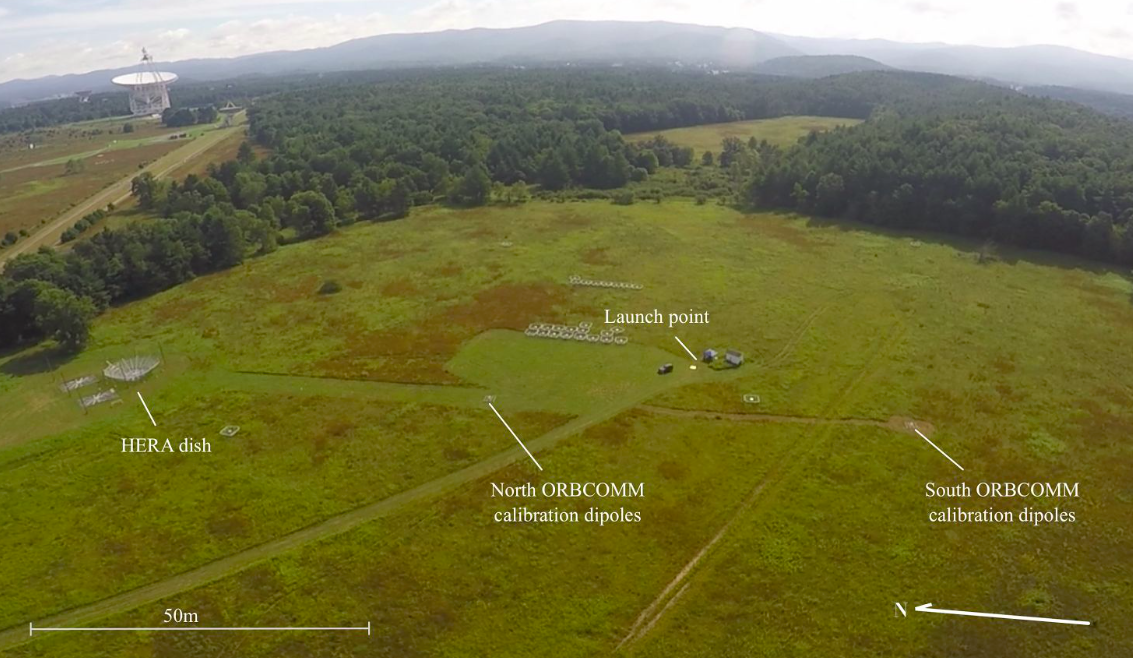
\includegraphics[width=6.5in]{aerial.png}
\caption{Aerial photograph of the two reference dipoles deployed in Galford Meadow at the National Radio Astronomy Observatory--Green Bank 100\,m south of the HERA dish.}
\label{fig:aerial}
\end{figure*}

\section{Assessing Systematics with a Null Experiment}

As in \citet{neben15}, we assess systematics using a ``null experiment'' in which we use a second reference dipole as the antenna-under-test (AUT). Taking the ratio of its measured power pattern with the model beam pattern amounts to a ratio of the row power responses received by the two antennas. This test thus probes the level of environmental systematics (i.e., reflections and varying ground properties) and antenna fabrication imperfections which affect each antenna differently. This is not a probe of modeling imperfections common to both antennas, but we expect such errors to be subdominant as the physical properties of the antenna are easier to characterize, and thus simulate, than local environmental effects. 

We run three null experiments with the reference dipoles deployed varying distances from the HERA dish and from each other.

\begin{itemize}
\item \texttt{null1}: reference dipoles deployed 50\,m apart on a NS line, 50\,m south of the HERA dish
\item \texttt{null3}: same as \texttt{null1} but with the south-most reference antenna moved 5\,m west
\item \texttt{null4}: same as \texttt{null1} but with 100\,m separation between both reference antennas and from the dish
\end{itemize}

Figure \ref{fig:null1} shows the results from the \texttt{null1} experiment in the form of the ratio of the power responses of the two antennas (top panel), and slices through the E an H planes of the reconstructed power patterns (bottom panel). We collected roughly 100 satellite passes. Systematics at the few percent level are observed in  within $20^\circ$ of zenith, and at the $\sim10\%$ level farther out.

The magnitude of these systematics is comparable to those observed in the two other null experiments (Figures \ref{fig:null3} and \ref{fig:null4}), an their angular distribution appears largely unchanged. This suggests that the reference dipoles differ both due to varying environmental properties and perhaps intrinsic differences. In any case, these fractional errors propagate directly into the measured beampatterns of our subsequent feed and dish measurements.  

\begin{figure*}[h]
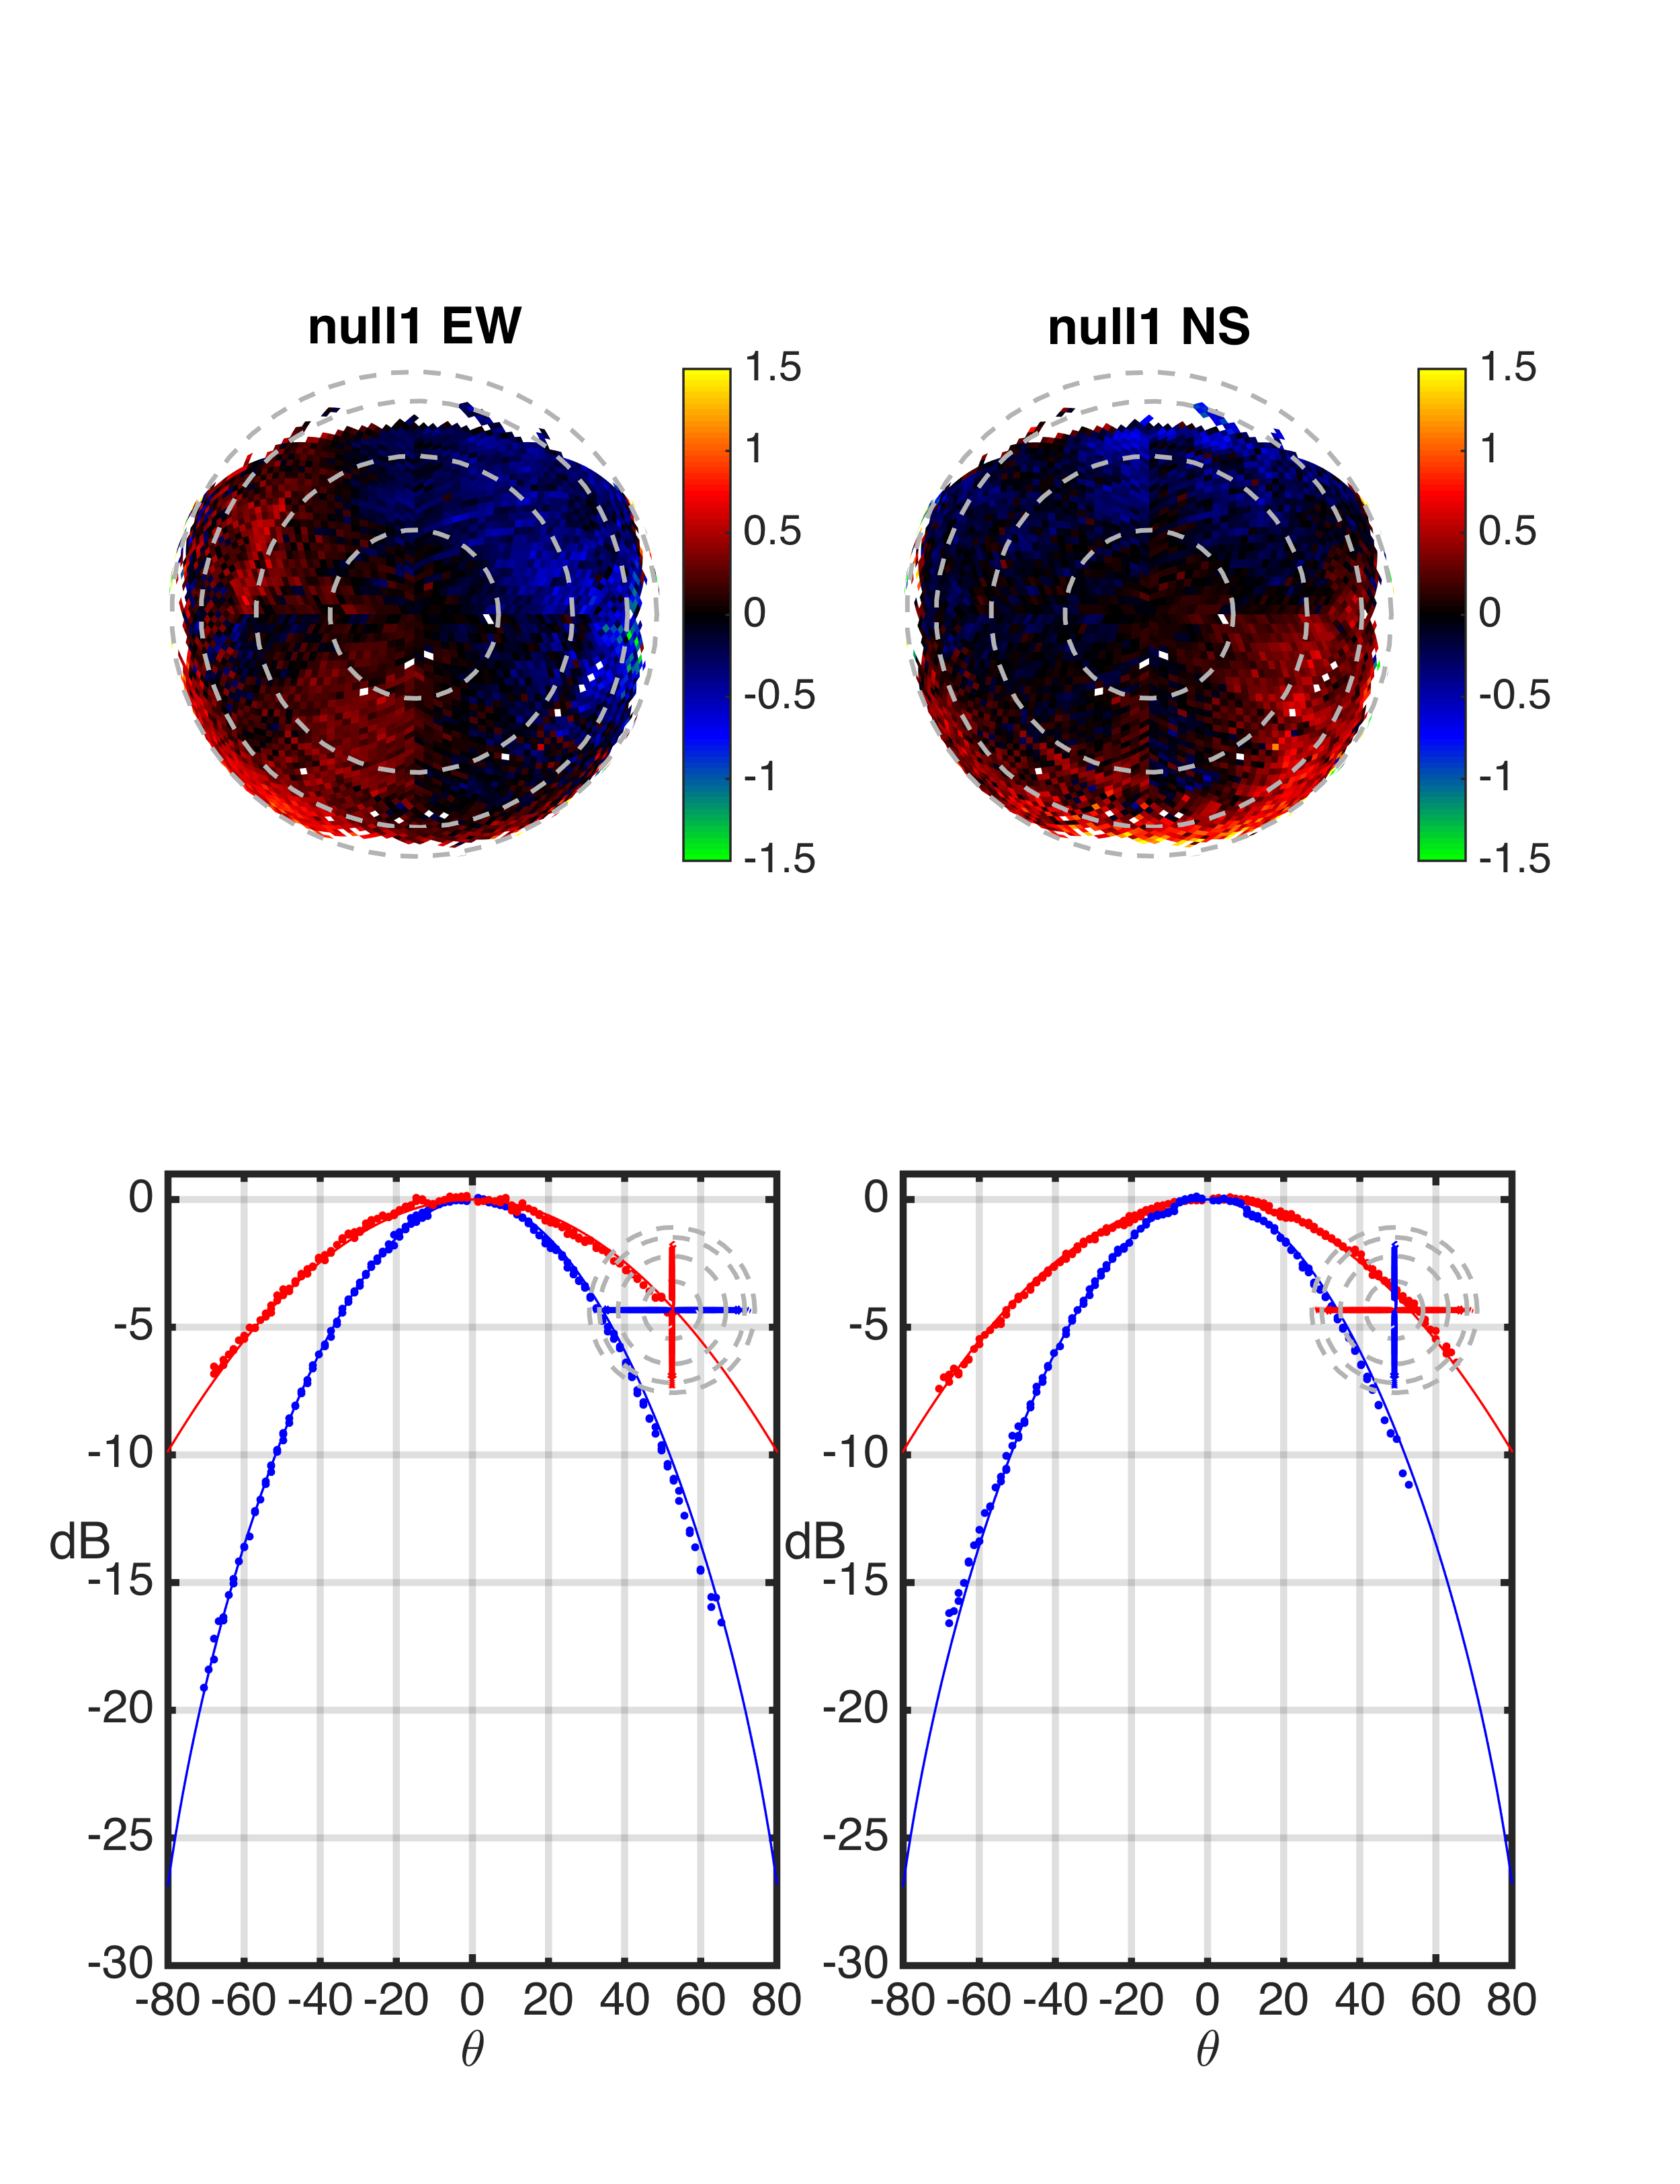
\includegraphics[width=6.5in]{null1_rel.png}
\caption{Top: ratio maps of the powers received by two reference dipoles separated by 50\,m, deployed 50\,m south of the HERA dish. Bottom: absolute beam power plots constructed by multiplying the relative power maps by a model beampattern. }
\label{fig:null1}
\end{figure*}

\begin{figure*}[h]
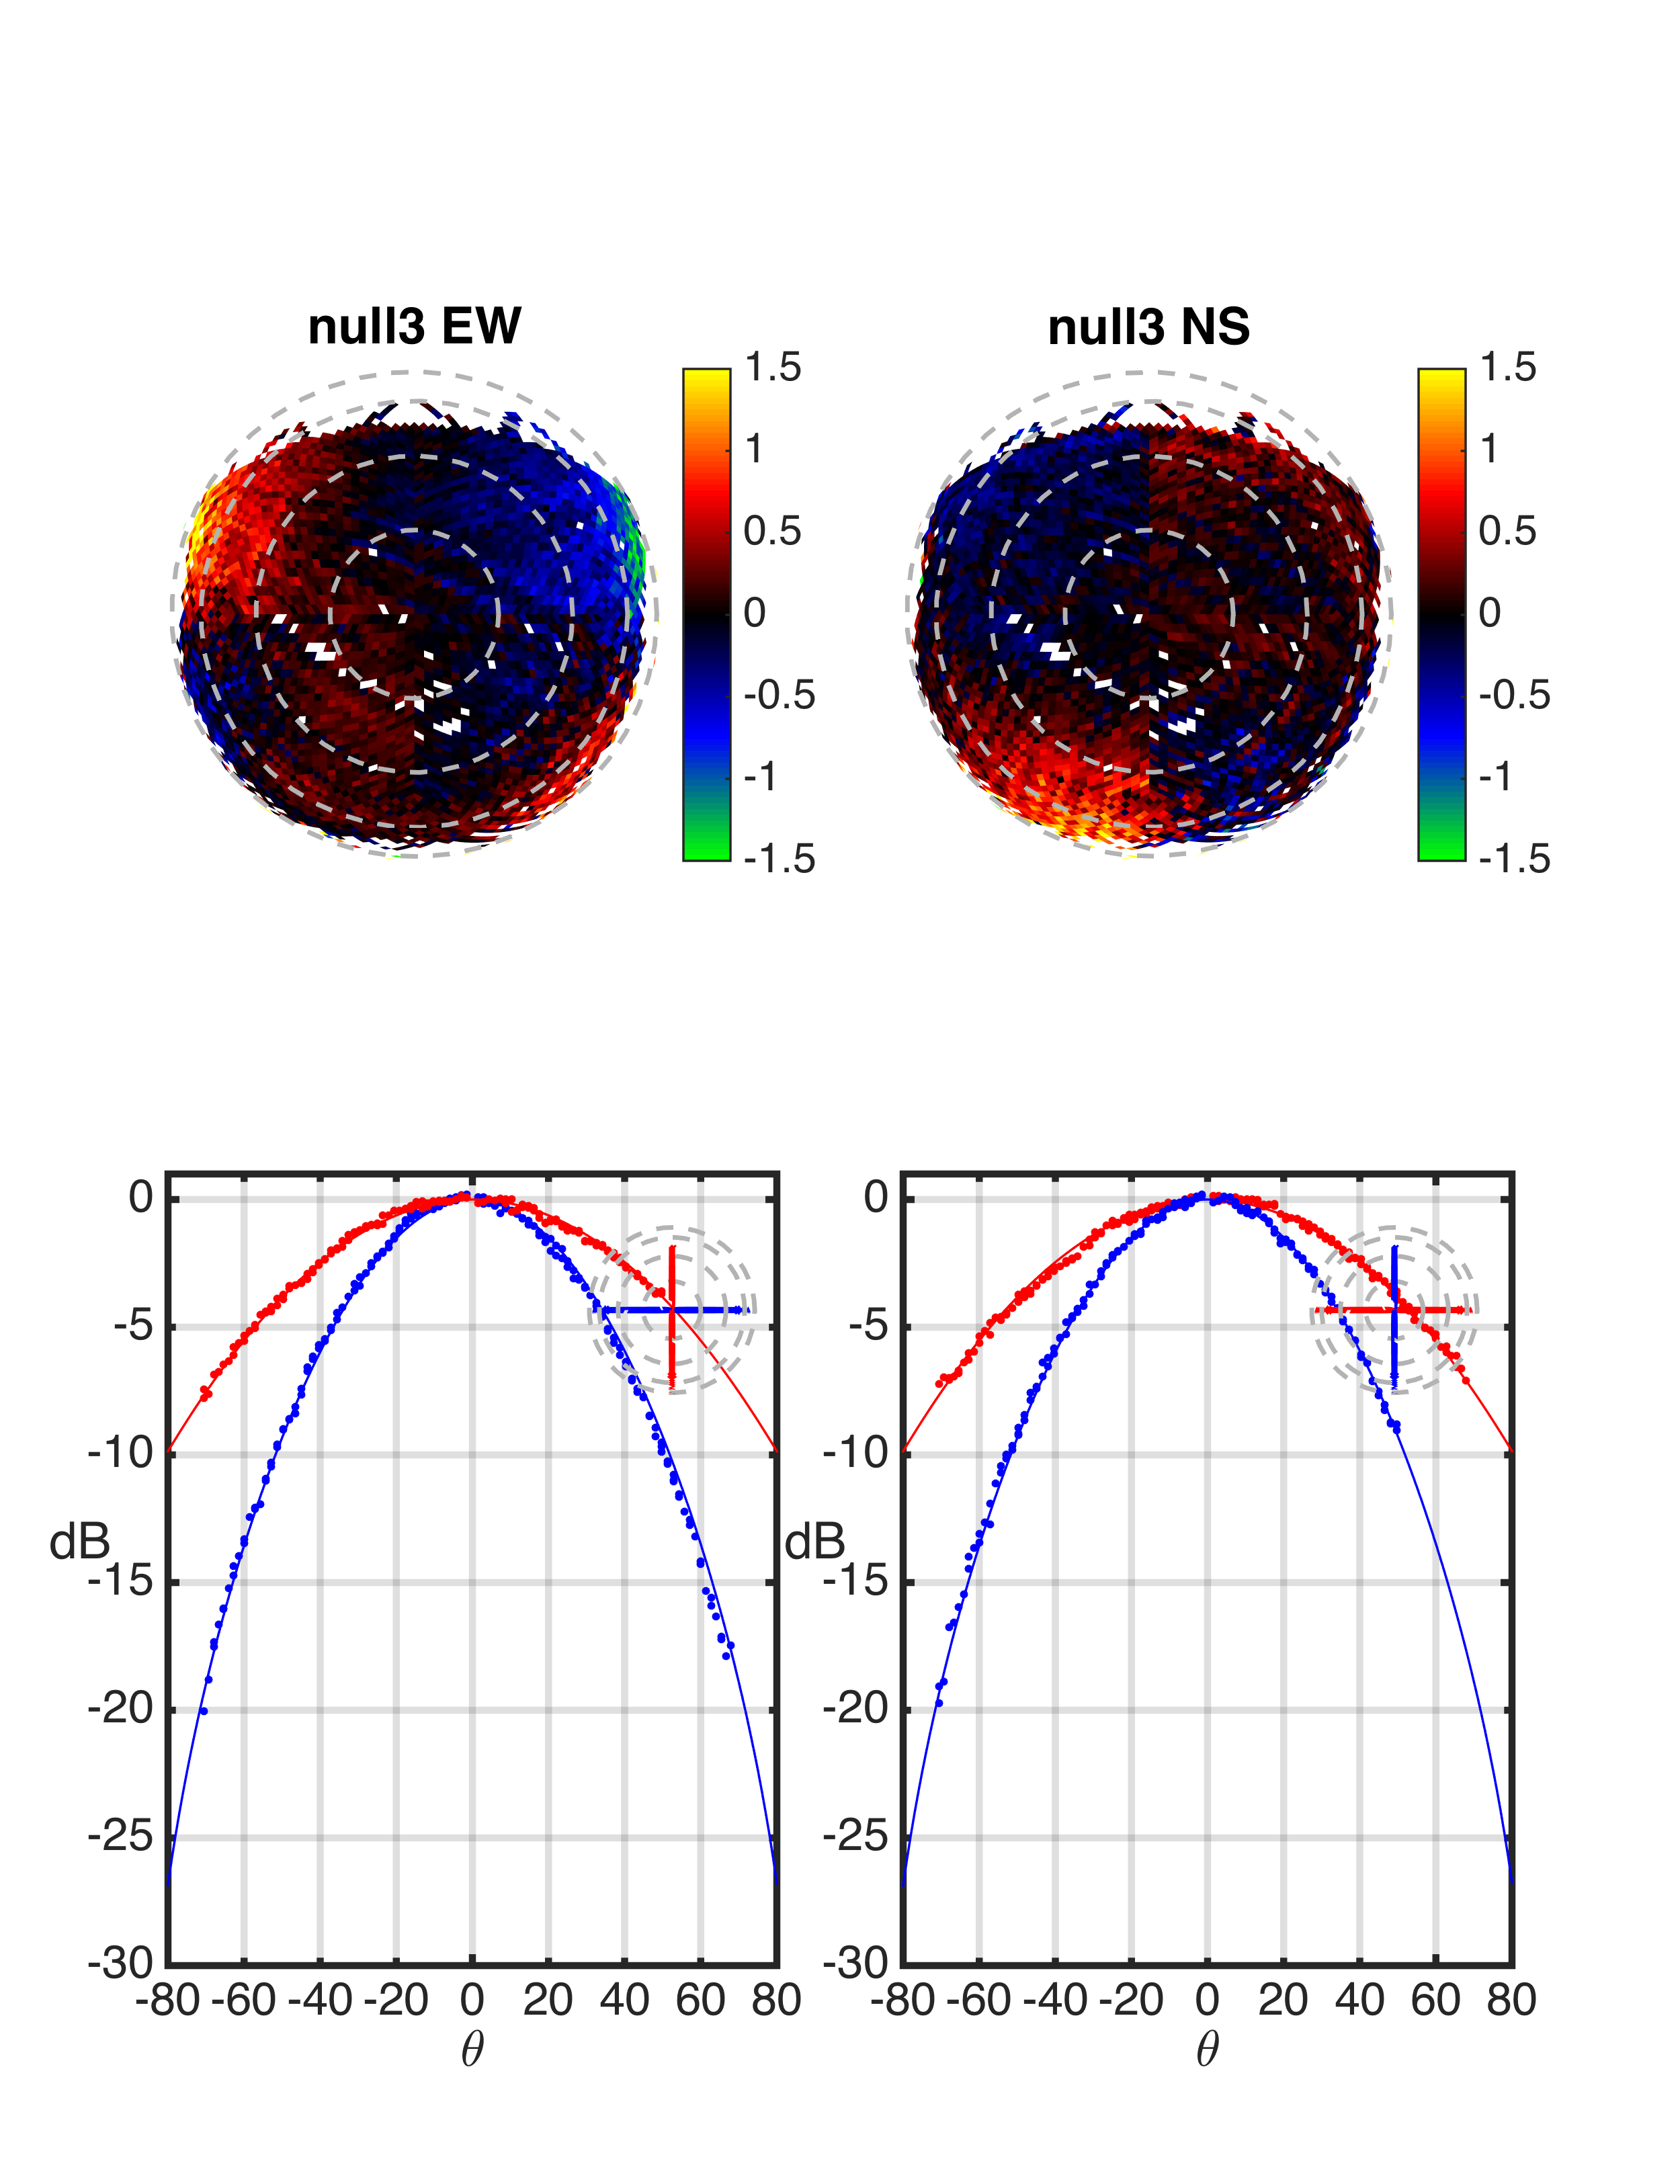
\includegraphics[width=6.5in]{null3_rel.png}
\caption{Same as the previous null experiment except the south reference dipole was moved 5\,m west. The systematics are largely unchanged.}
\label{fig:null3}
\end{figure*}

\begin{figure*}[h]
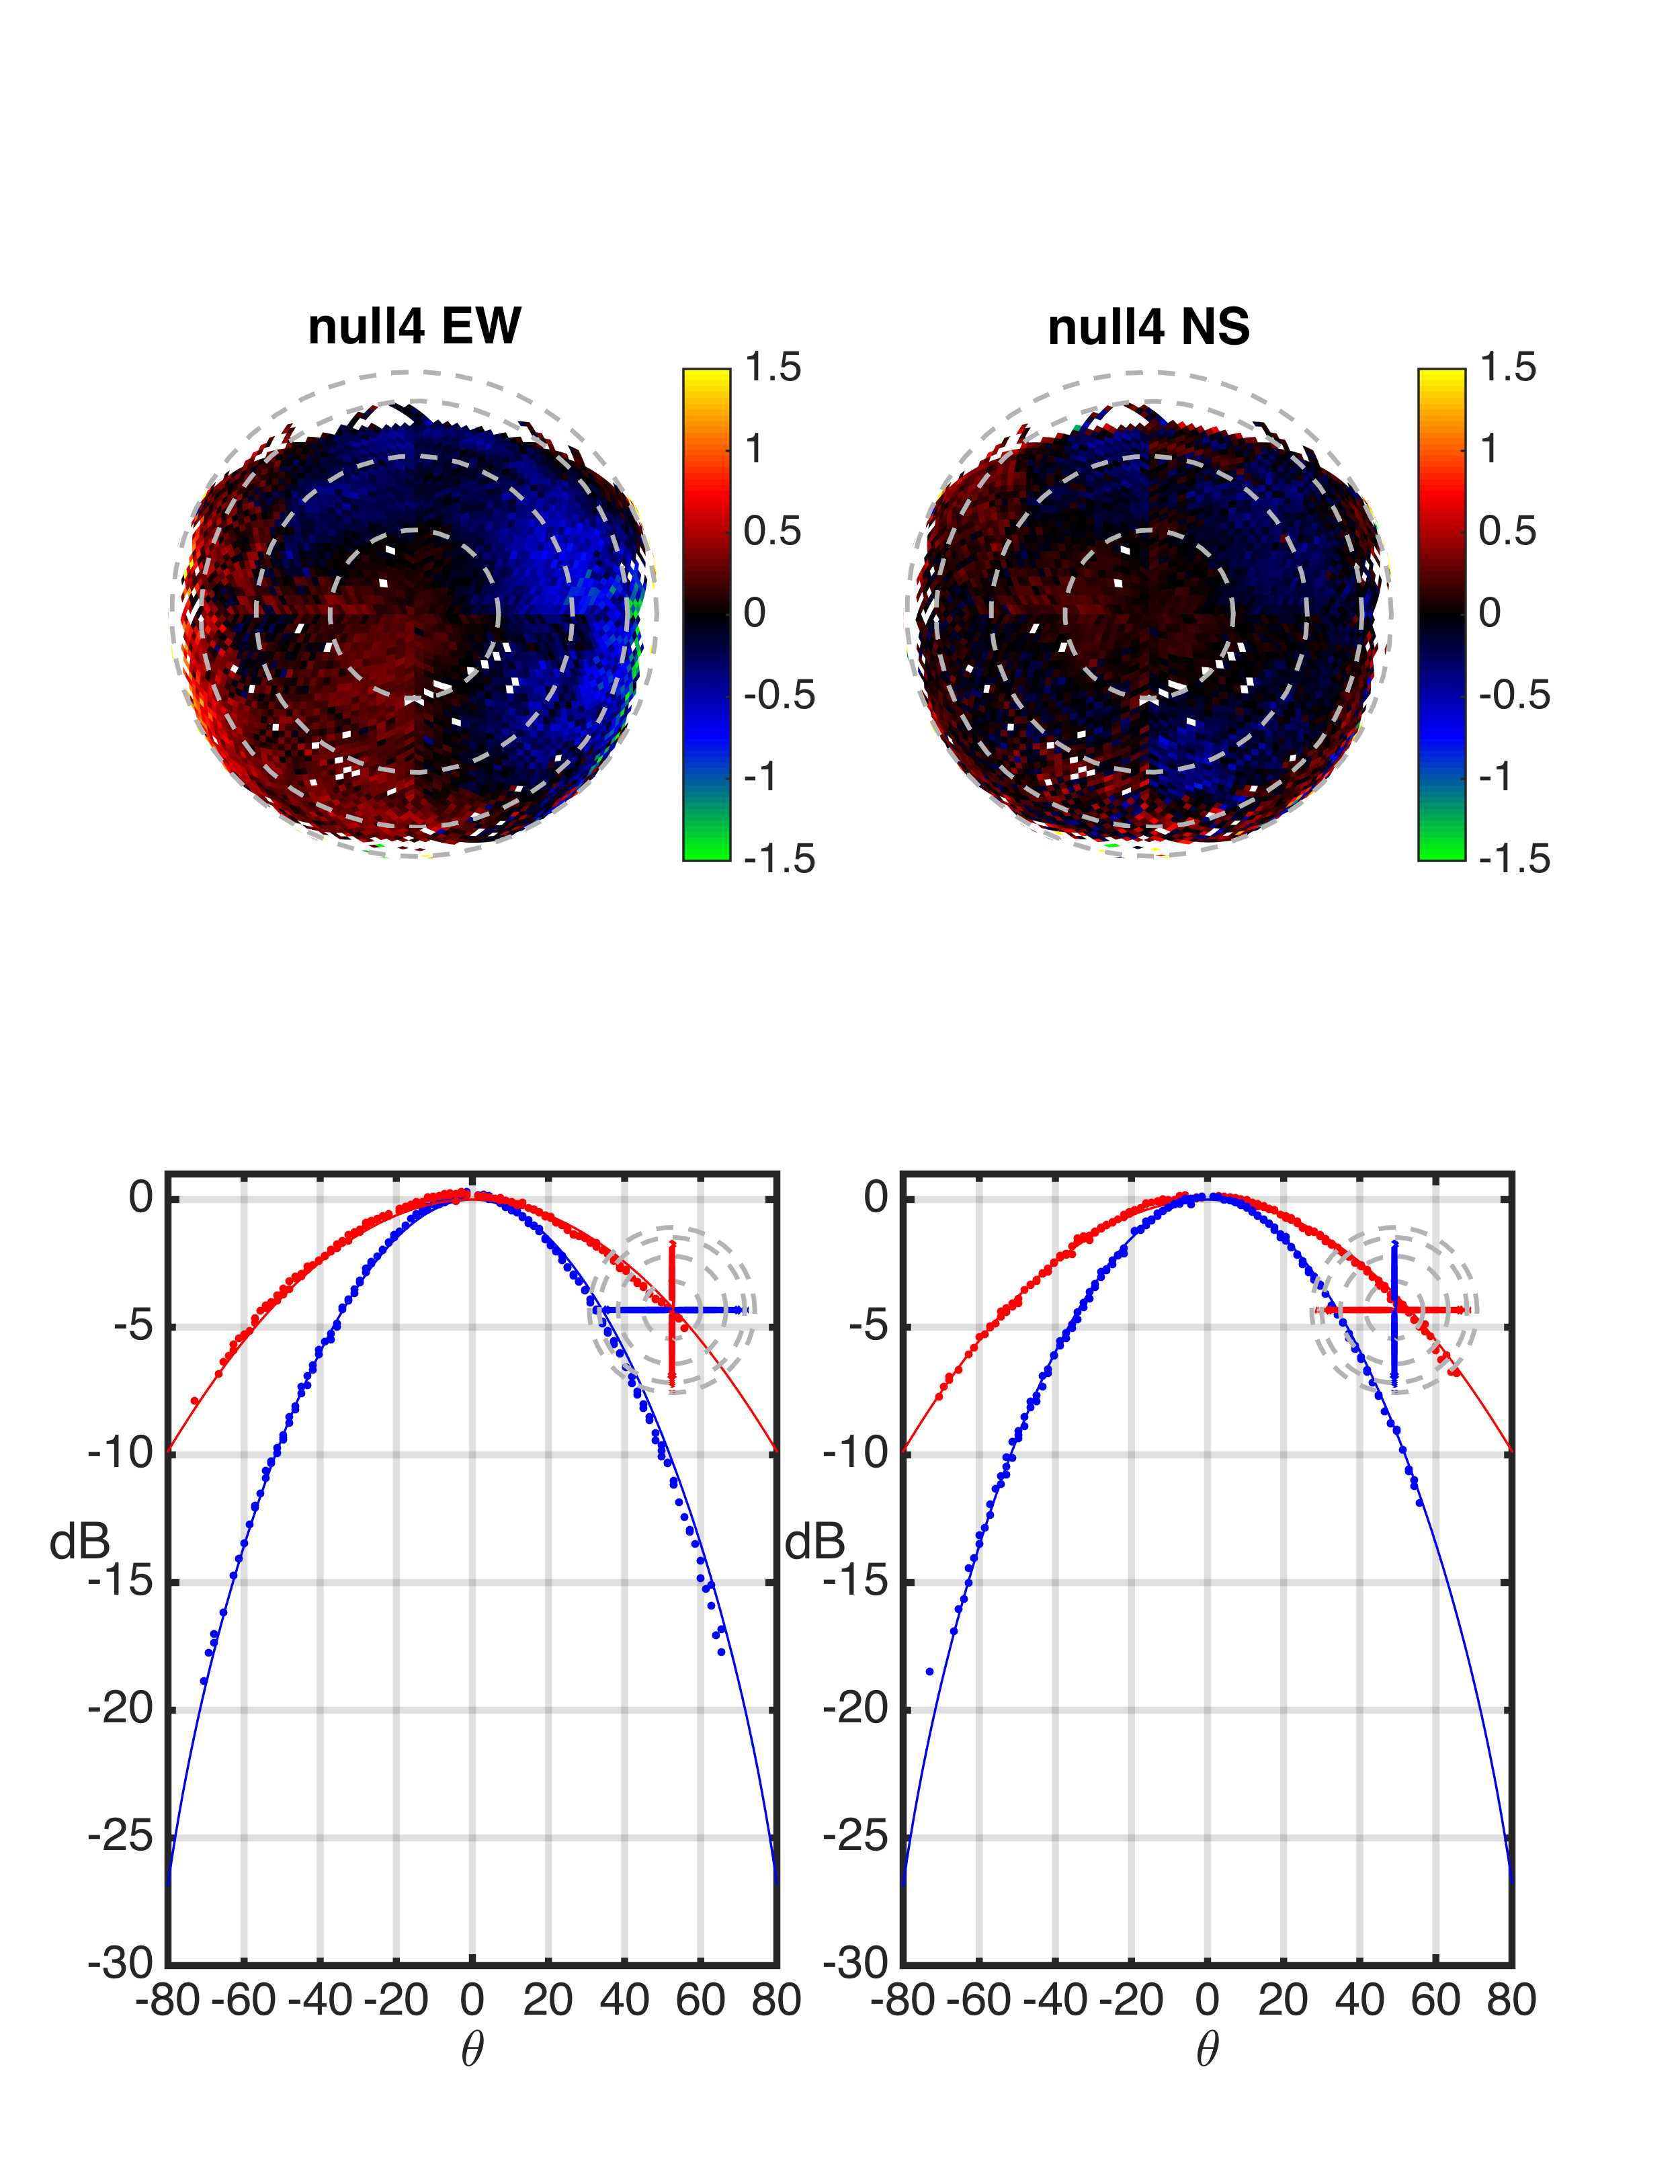
\includegraphics[width=6.5in]{null4_rel.png}
\caption{Same as the first null experiment except the reference dipoles are separated by 100\,m and deployed 100\,m south of the HERA dish. The systematics remain at the few percent level near zenith and increase to $\sim10\%$ farther out, with somewhat, but not entirely different angular structure. }
\label{fig:null4}
\end{figure*}

\section{Feed Measurements}

Accurate modeling of both the dish and feed will be essential for final dish modeling. To that end, we deploy the feed on the ground facing the sky (Figure \ref{fig:feedpic}), replacing the north-most reference antenna in the \texttt{null3} configuration, to isolate the feed power pattern. 

Figure \ref{fig:feed0} shows the measured feed beams (top panel) and slices through the E and H planes (bottom panel). Due to intermittent connection problems to the DAQ computer, we collected only 157 high signal-to-background satellite passes over a few days. Still, the data agree very well with the CST model for $\theta<55^\circ$, outside of which the E plane response starts narrows compared to the model by up to 5\,dB at $\theta=70^\circ$. Still, the data are quite sparse in these low regions due to the connection problems, and so the usual quality control cuts are likely less effective than usual. 

\begin{figure*}[h]
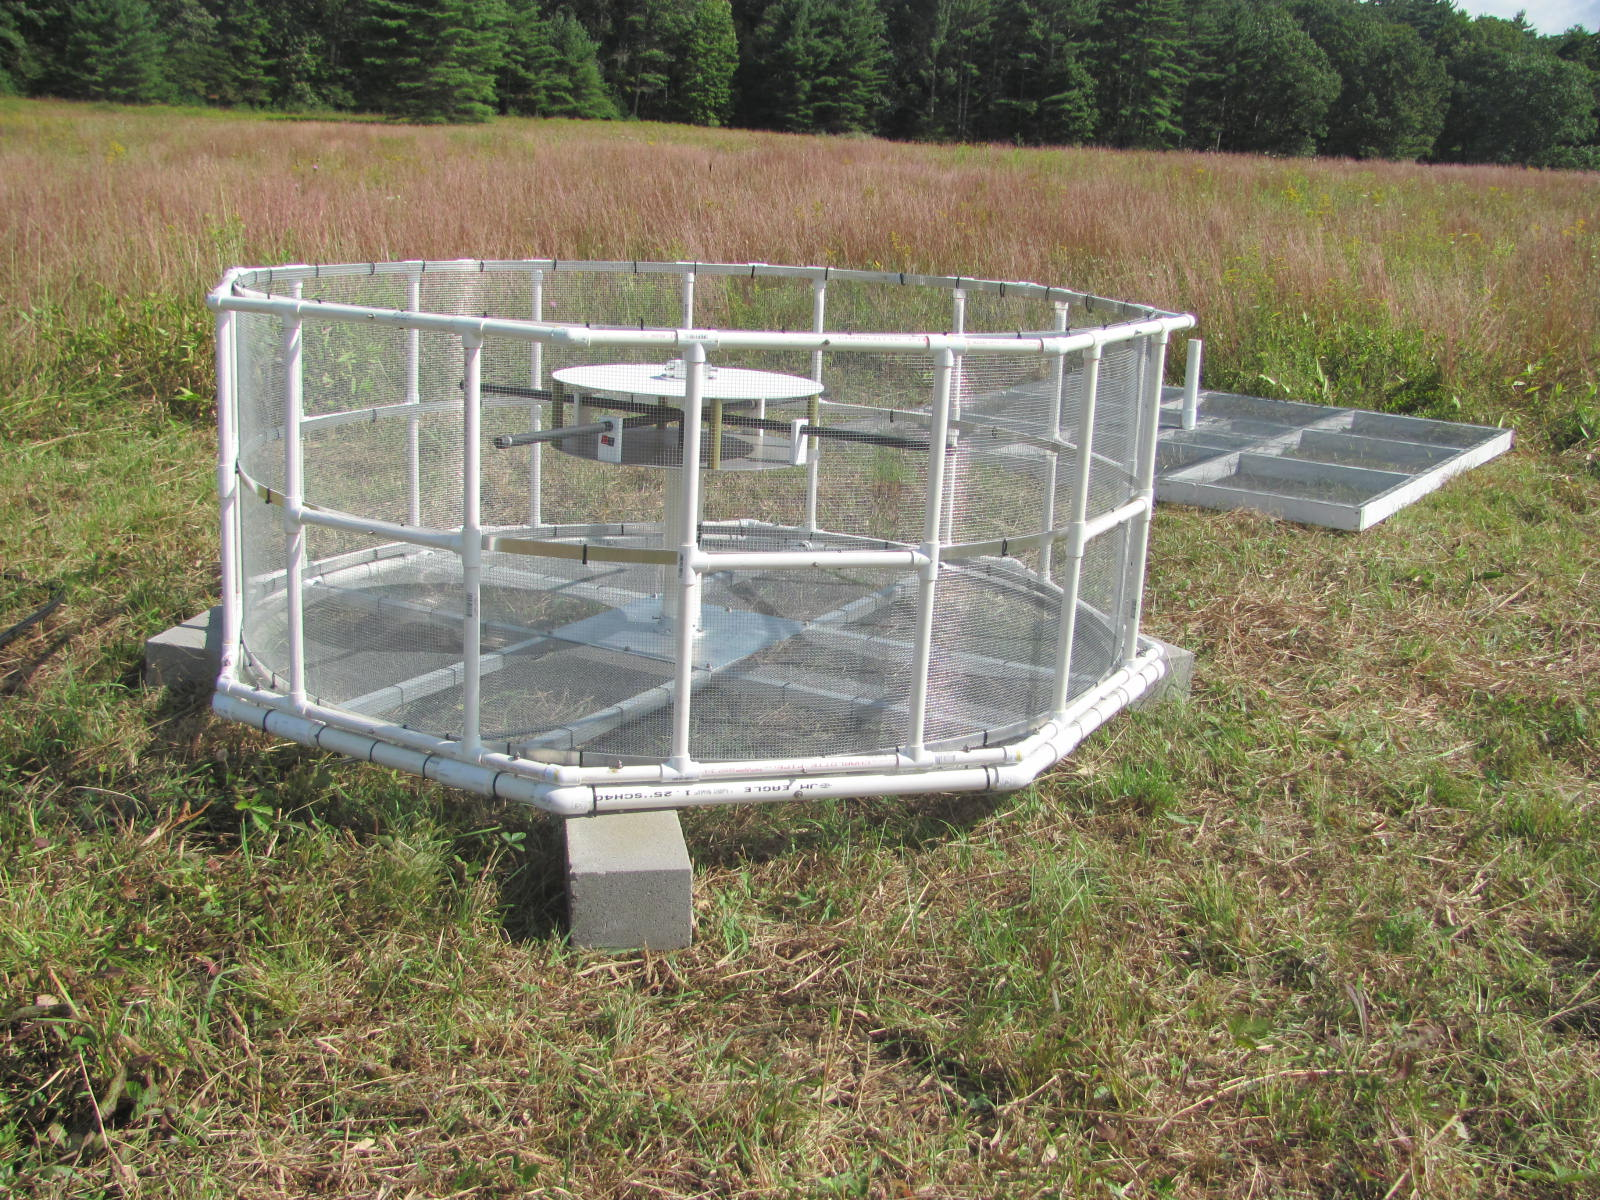
\includegraphics[width=5in]{feed.jpg}
\caption{Feed deployed on the ground, facing the sky, replacing the north-most reference antenna in the \texttt{null3} configuration. }
\label{fig:feedpic}
\end{figure*}

\begin{figure*}[h]
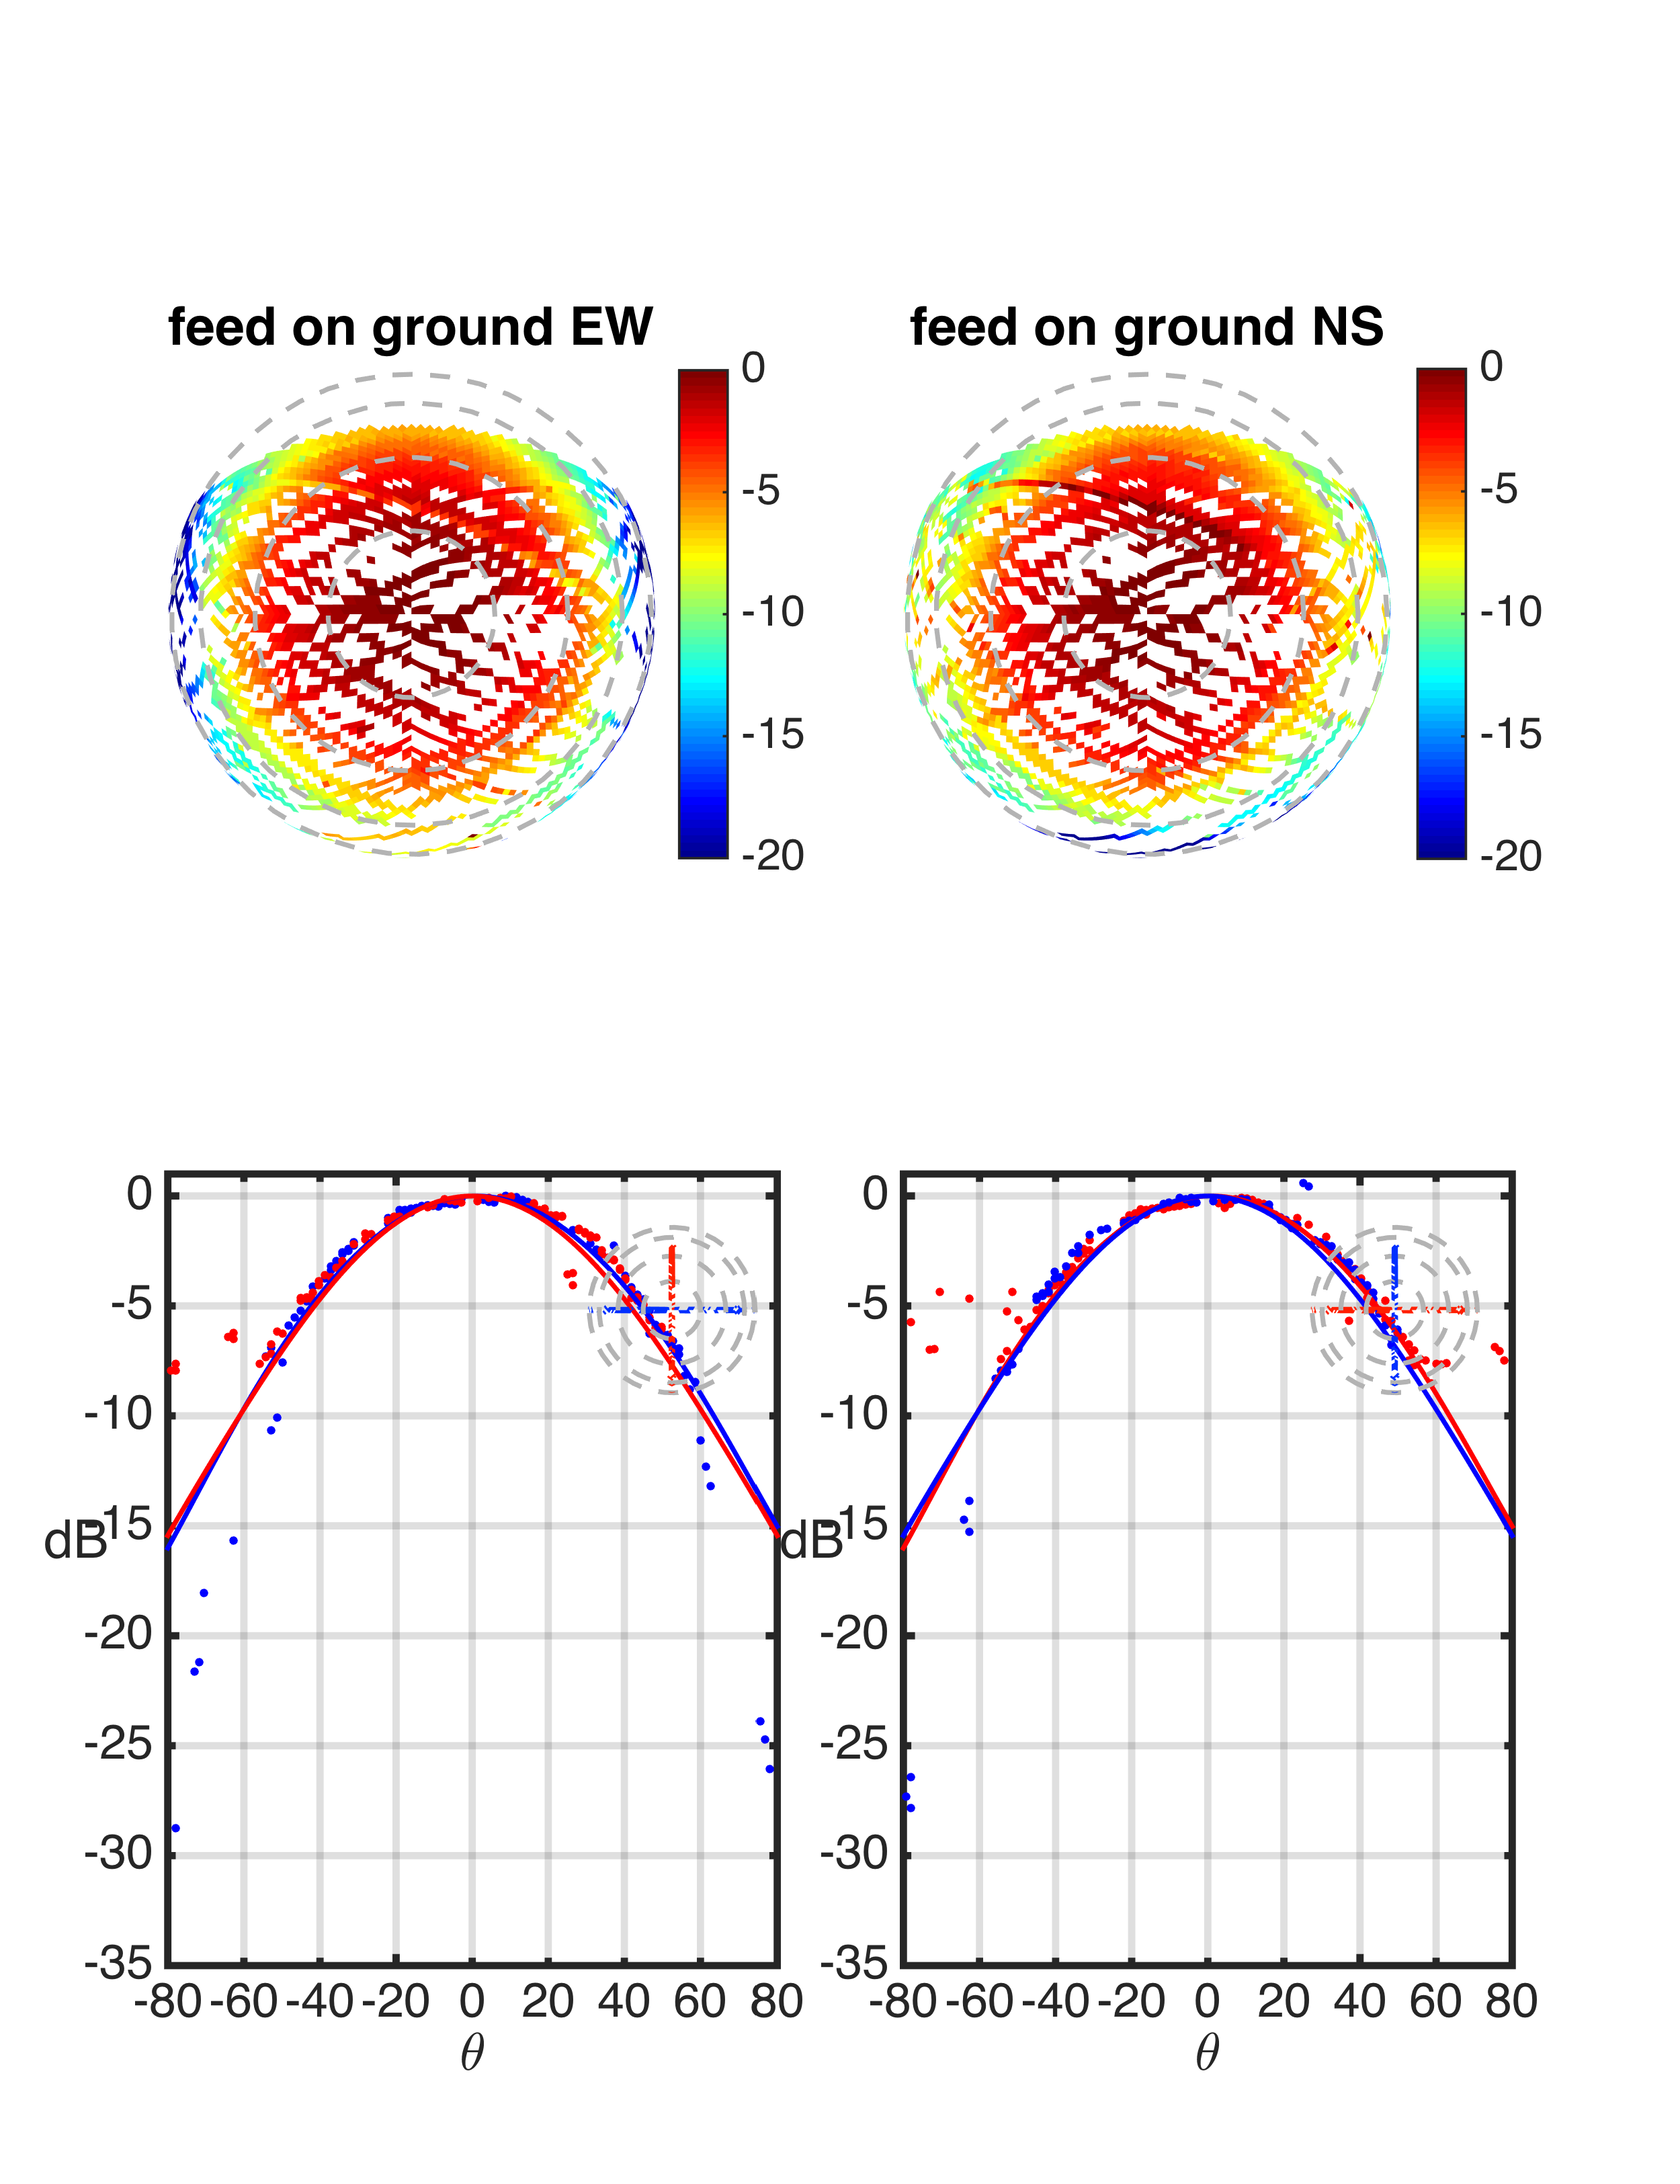
\includegraphics[width=6.5in]{feed0_abs_old_ref_model.png}
\caption{Measurements of the feed power pattern, deployed so it faces the sky. The measurements agree well with the model for $\theta<55^\circ$, but start to diverge at large zenith angles, possibly due to quality control problems due to very sparse beam sampling.}
\label{fig:feed0}
\end{figure*}

\section{Dish Characterization}

\subsection{Power pattern measurements}

Having verified the feed power pattern, we deployed feed over the dish and proceed with dish measurements. We measure the power pattern with the feed at four different heights, 4\,m, 4.5\,m, 5\,m, and 5.3\,m, chosen to probe around the nominal focus of 4.5\,m (the nominal beam) and up to the maximum height of 5.3\,m allowed by pole height and rope stresses. Heights are measured from the dish surface to the feed backplane. 

Inspecting the E and H plane slices through the measured beams (bottom panels) in Figures \ref{fig:dish3}, \ref{fig:dish1}, \ref{fig:dish2}, \ref{fig:dish4}, we generally see the main lobe narrow and the sidelobe level decrease. The improvement is also seen in the yellow and red main lobe in the beam maps (top panels) which narrow and approach the expected orientations: the EW (NS) main lobe is elongated in the NS (EW) direction. The last lift produced the smallest change in the beam suggesting it is quite near the best focus. 

The sky coverage in these dish measurements extends out to typically $\theta\sim50-60^\circ$. Beyond that the ORBCOMM flux is sufficiently attenuated relative to diffuse galactic emission that a power ratio measurement between the two antennas is no longer a clean probe of their gains in the direction of the satellite. At these zenith angles, the beam sidelobes are roughly -30\,dB, and seem to be trending downward at the edge of the measured region.

\begin{figure*}[h]
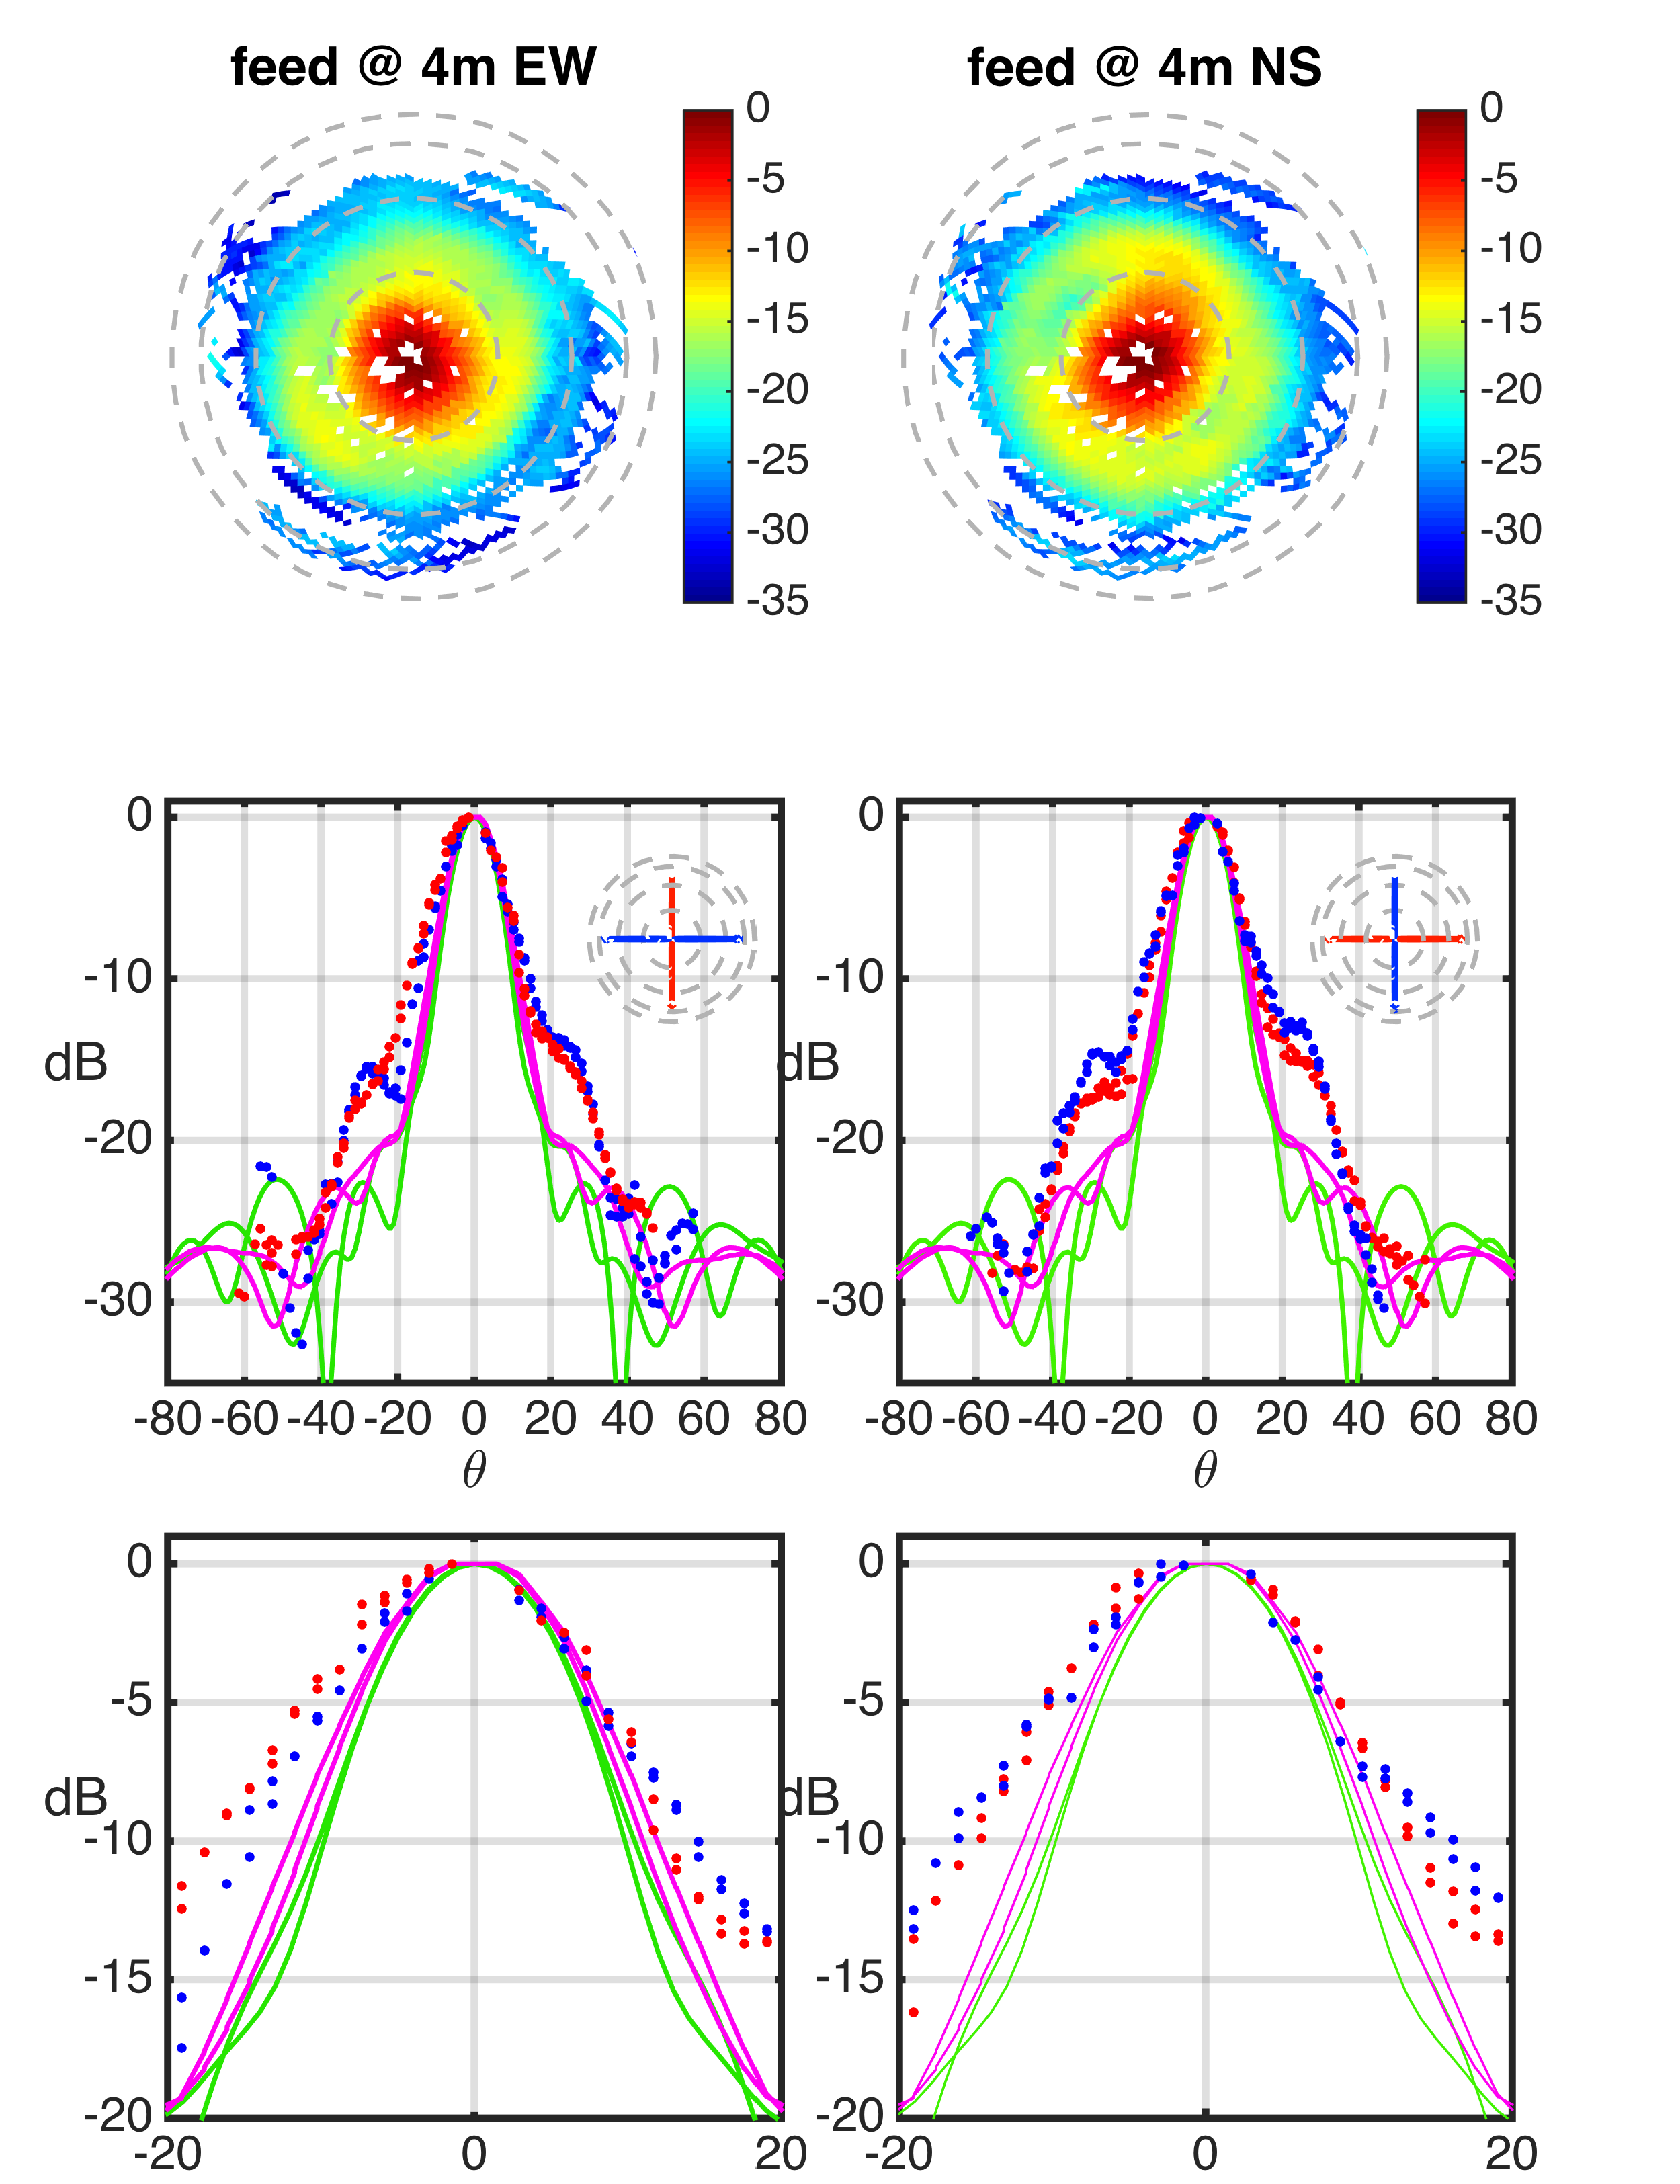
\includegraphics[width=6.5in]{dish3_abs_old_ref_model.png}
\caption{Dish power pattern with the feed lowered 0.5\,m below nominal focus.}
\label{fig:dish3}
\end{figure*}

\begin{figure*}[h]
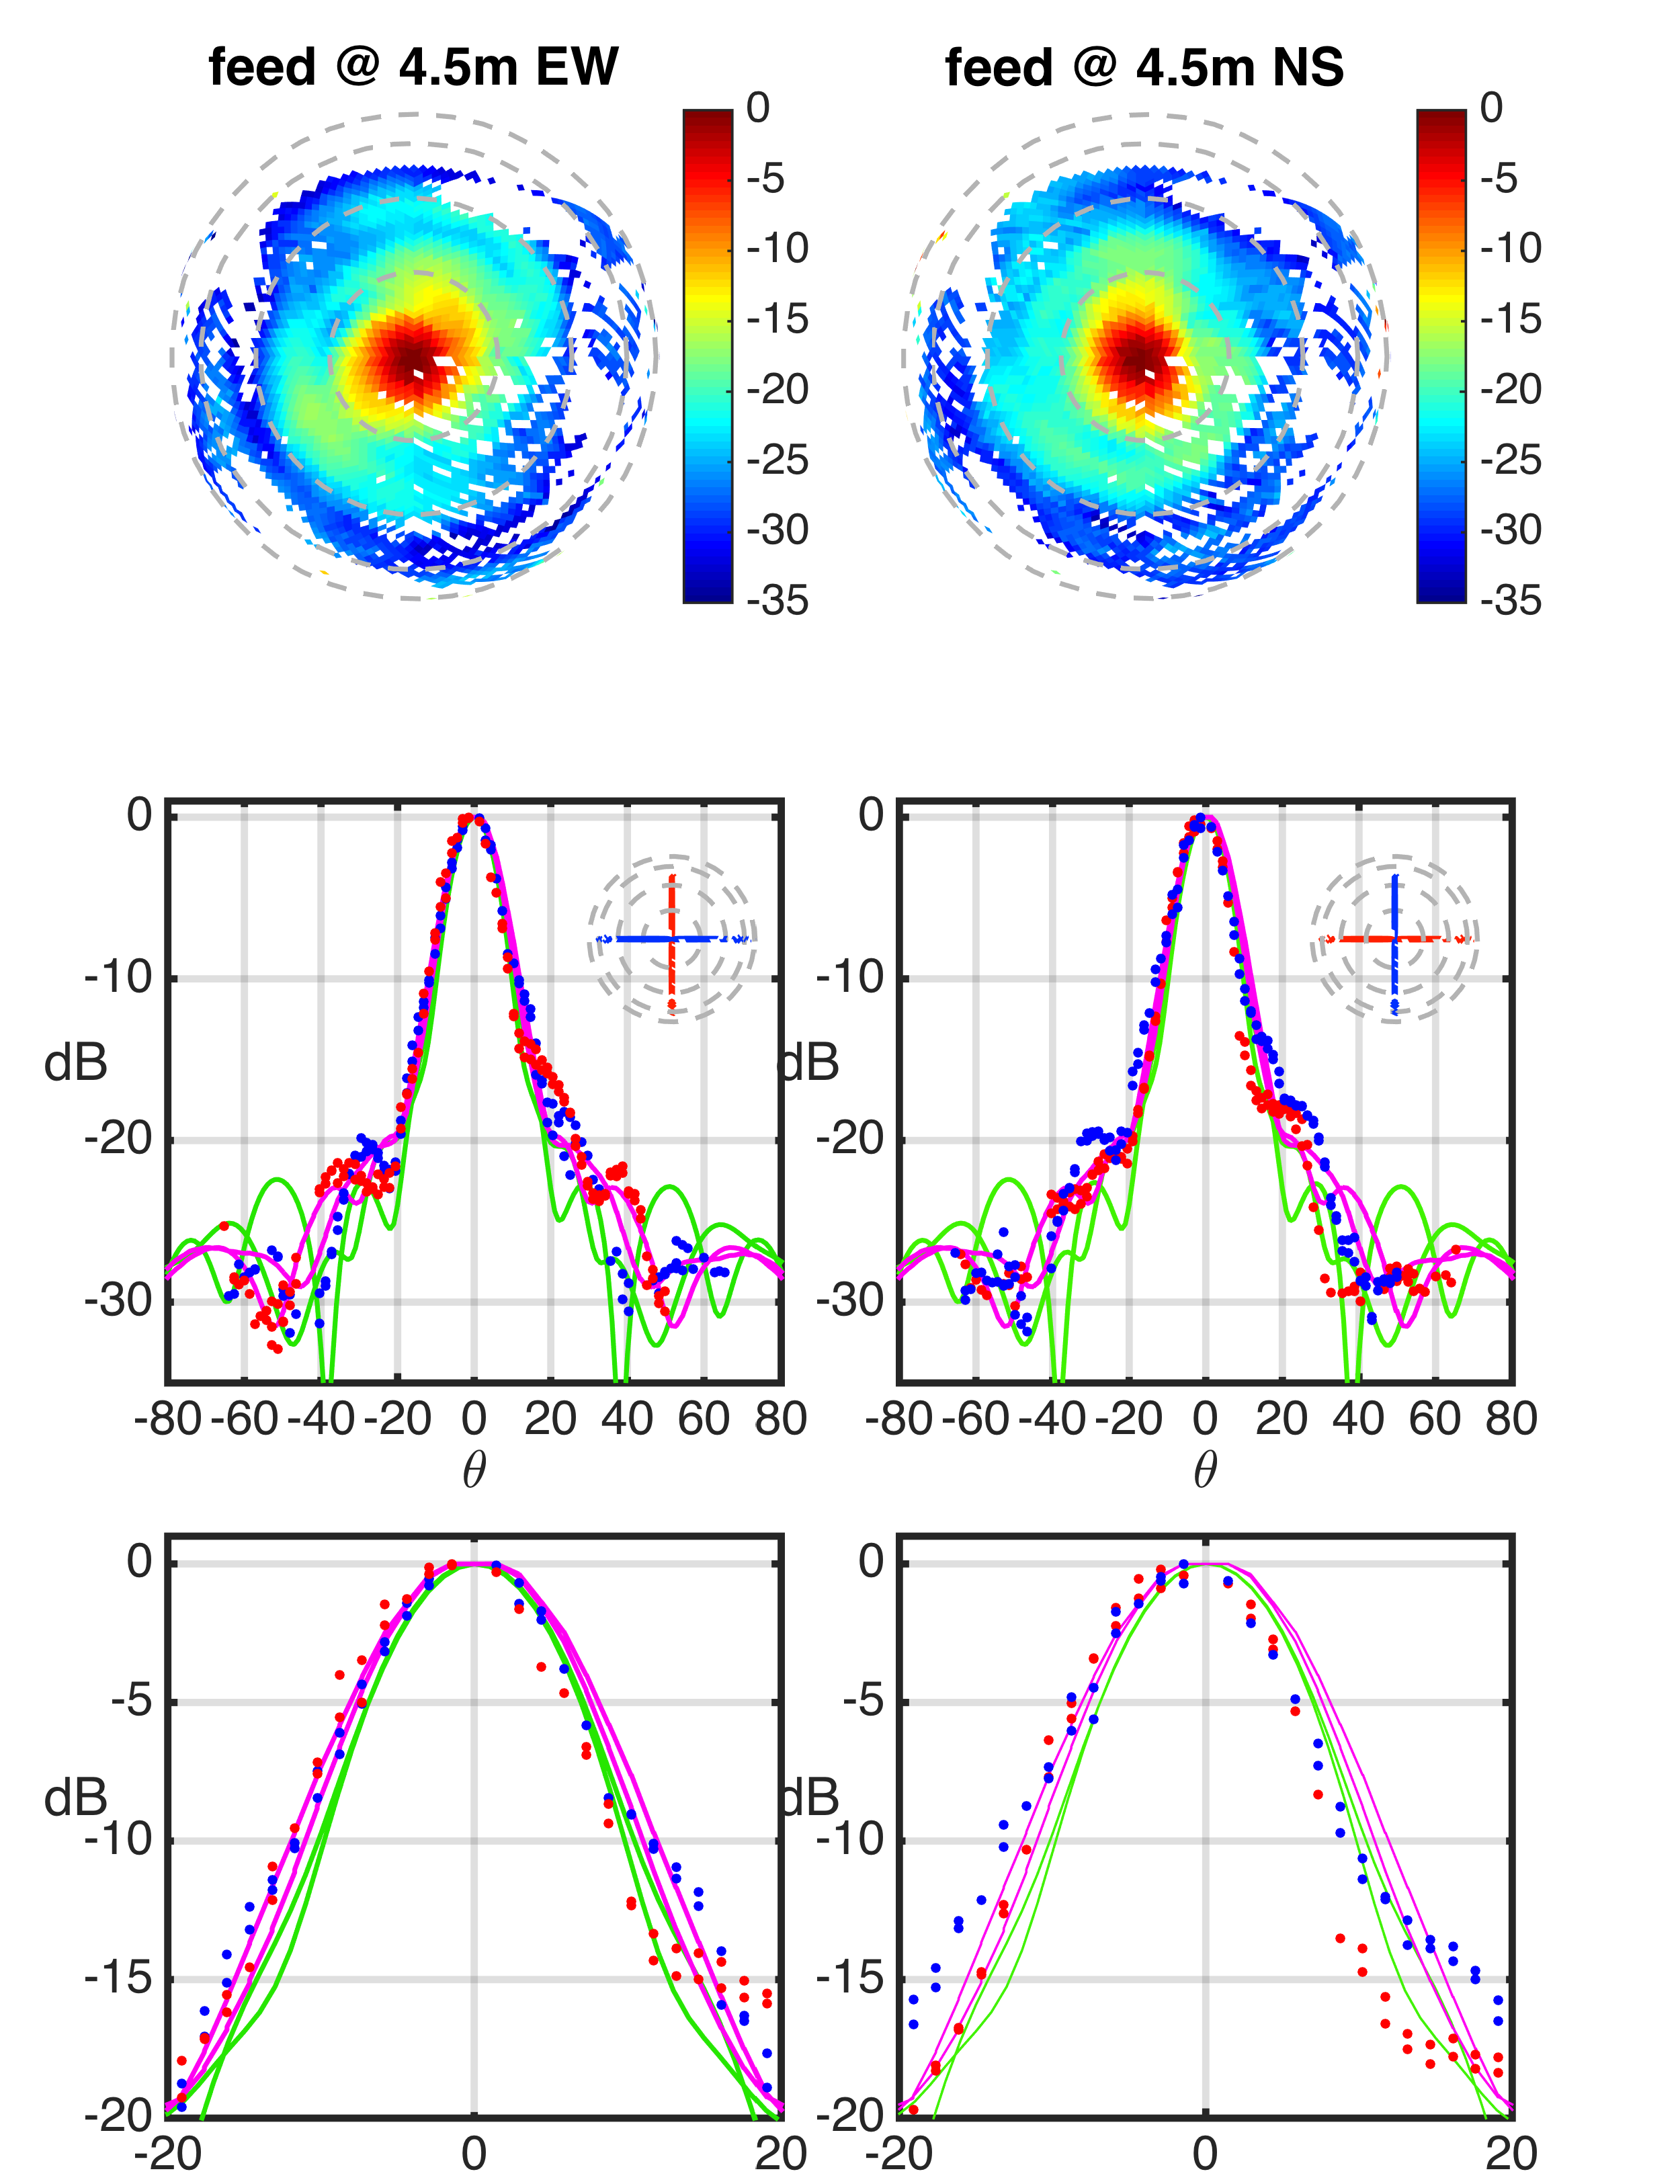
\includegraphics[width=6.5in]{dish1_abs_old_ref_model.png}
\caption{Dish power pattern with the feed at the nominal focus of 4.5\,m.}
\label{fig:dish1}
\end{figure*}

\begin{figure*}[h]
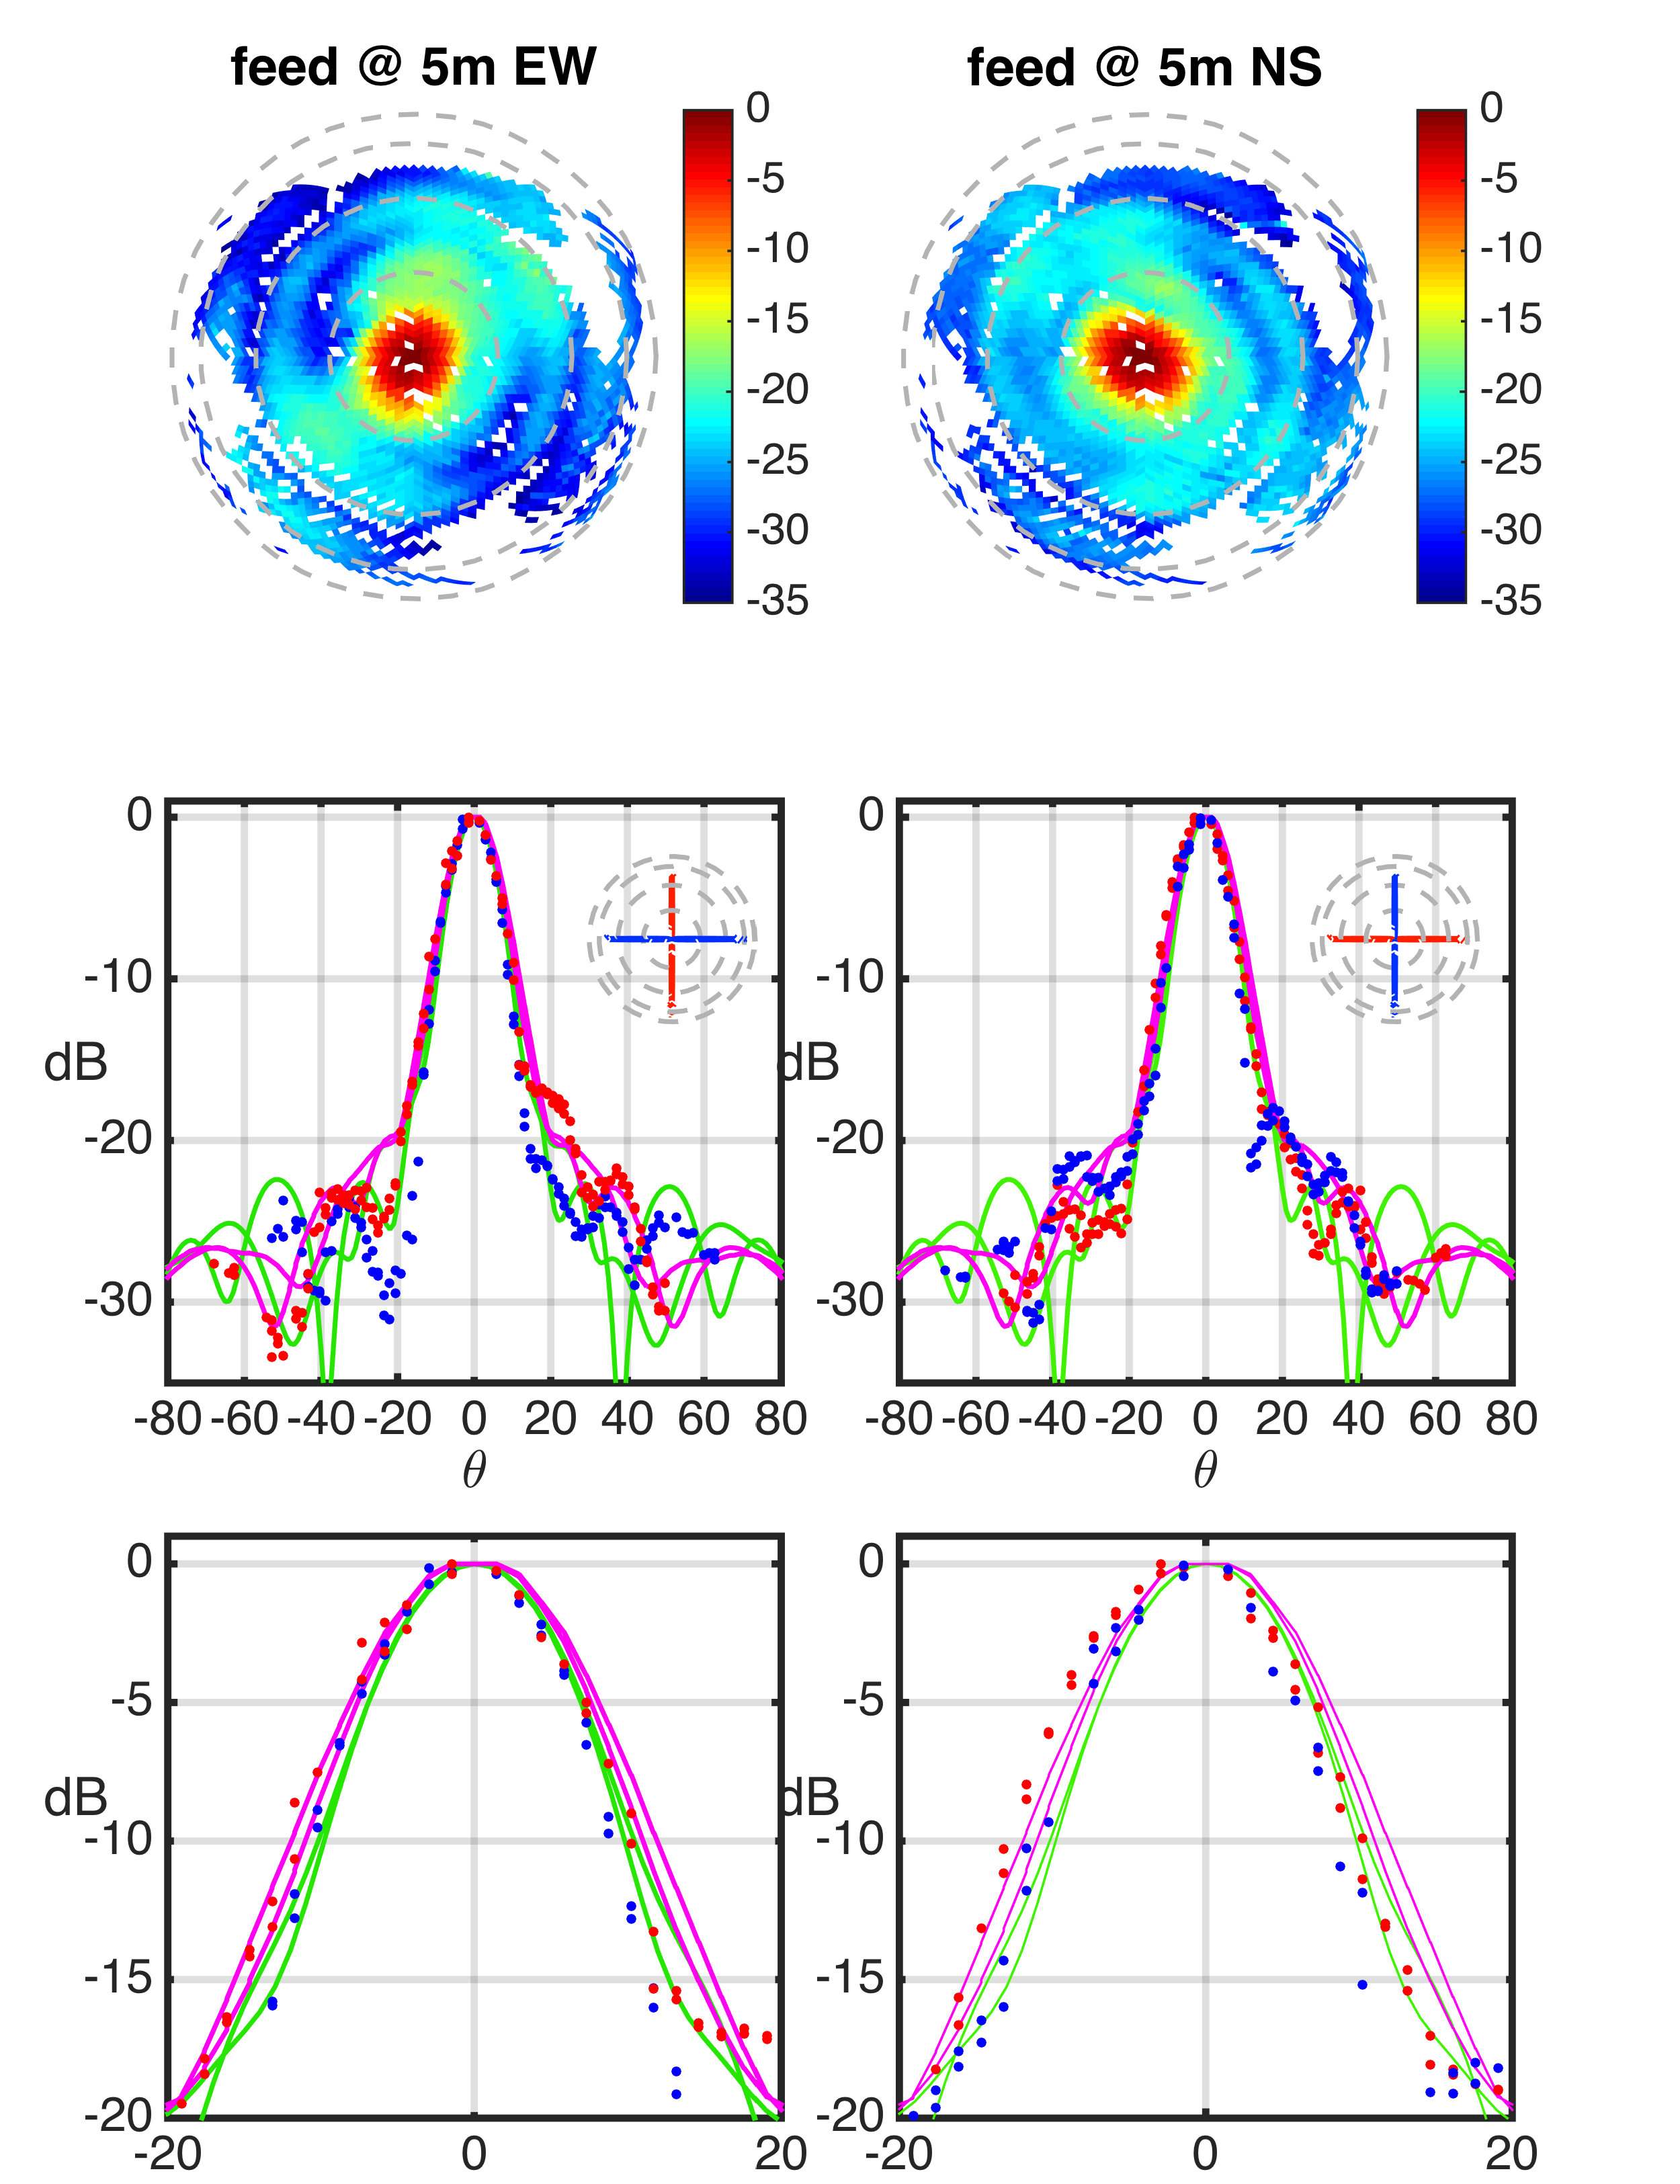
\includegraphics[width=6.5in]{dish2_abs_old_ref_model.png}
\caption{Dish power pattern with the feed raised 0.5\,m above nominal focus.}
\label{fig:dish2}
\end{figure*}

\begin{figure*}[h]
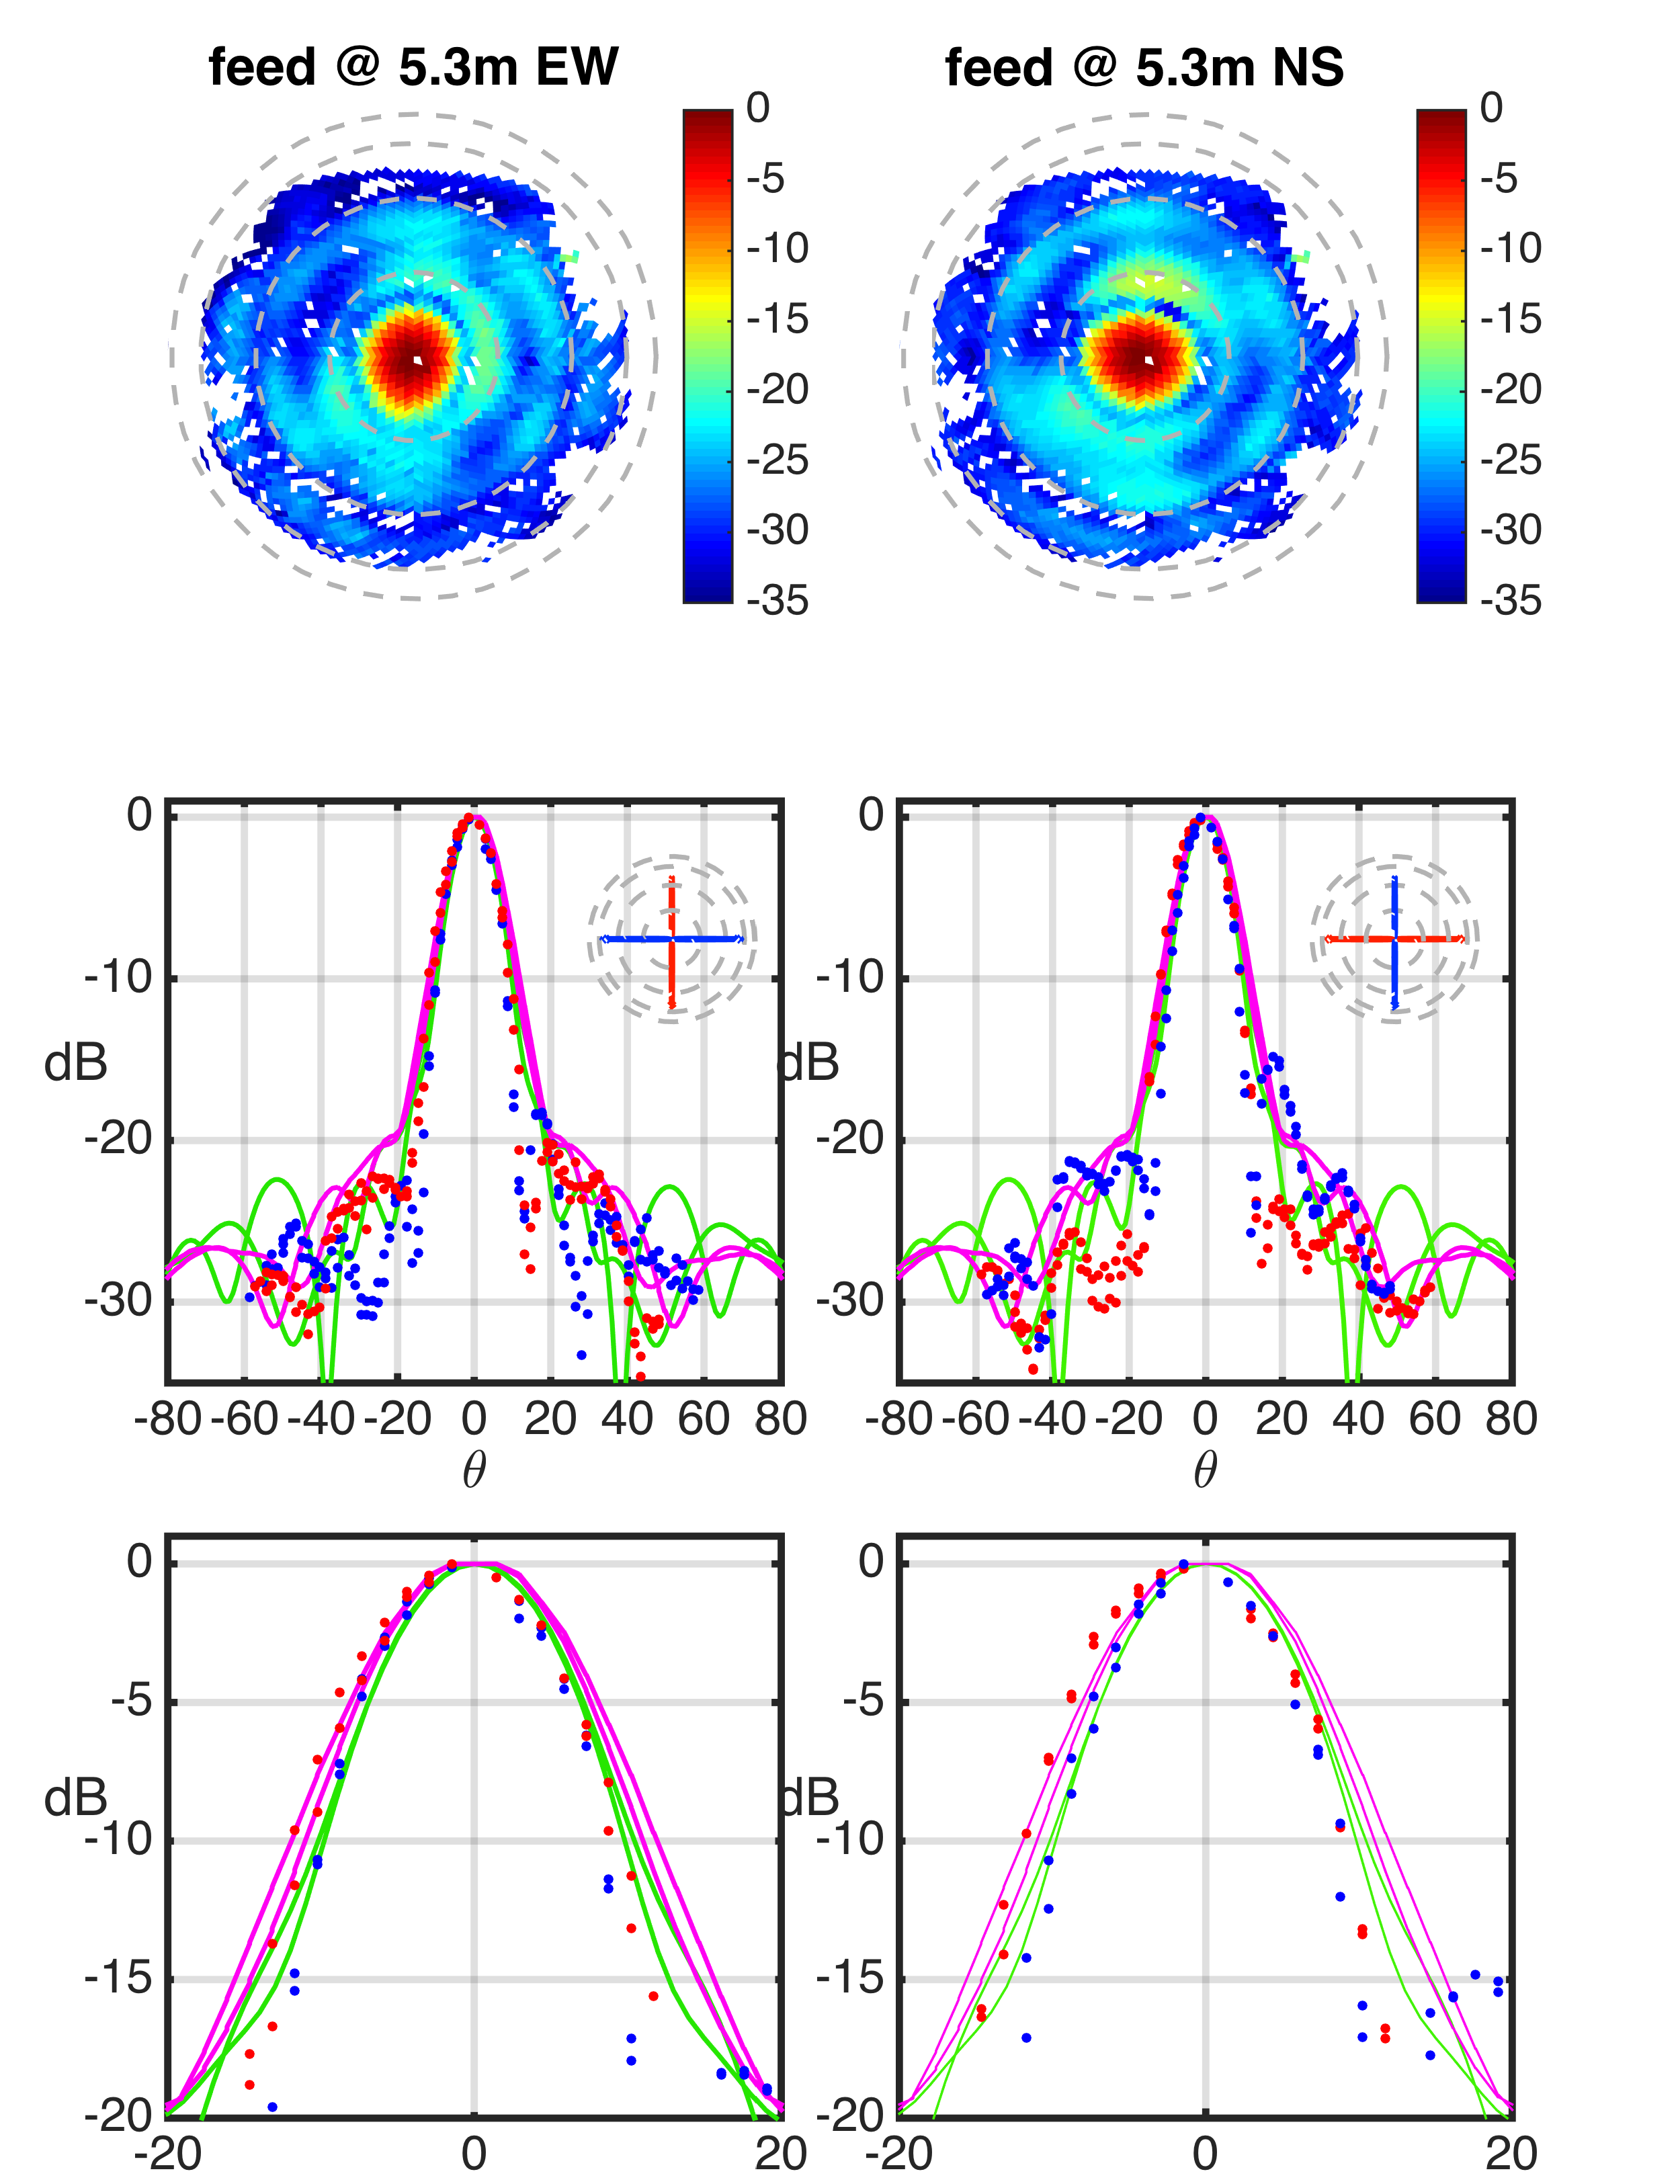
\includegraphics[width=6.5in]{dish4_abs_old_ref_model.png}
\caption{Dish power pattern with the feed raised to its maximum height of 0.8\,m above nominal focus.}
\label{fig:dish4}
\end{figure*}

In order to compute beam collecting areas and assess foreground leakage we require a beam covering the entire visible sky. For each measured dish beam, we interpolate over the unmeasured cells at $\theta\lesssim60$, then extrapolate outward to the horizon. This amounts to a smooth continuation of the beam response at the same $\sim-30$\,dB level suggested by the fringes of our measurements. We take this as a first possible model of the full sky dish beam, and construct a second with a gaussian cutoff at $\theta=60^\circ$ with $\sigma=2.5^\circ$, the pair of which span the space of likely horizon responses. This procedure is depicted in Figure \ref{fig:interpbeams} where we plot the measured nominal focus beam, the beam after interpolation and extrapolation, and the beam after applying the gaussian cutoff. Figure \ref{fig:interpbeamsslice} shows the interpolated/extrapolated beam and the beam with the cutoff along with various models to illustrate the different horizon responses more clearly.

\begin{figure}[h]
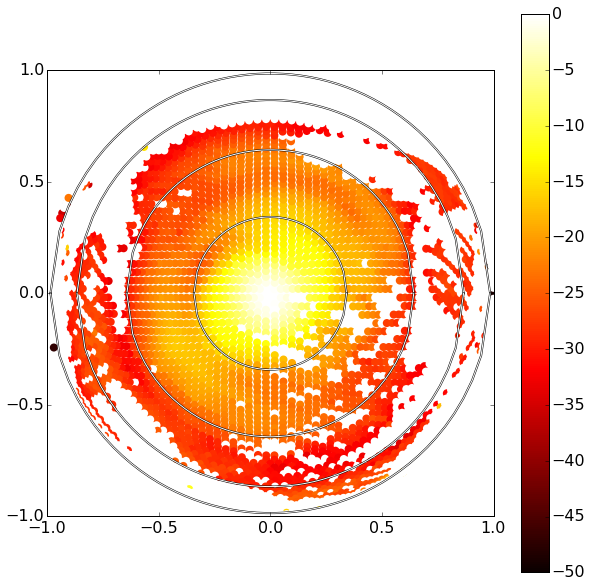
\includegraphics[width=3.5in]{measbeam_raw.png}
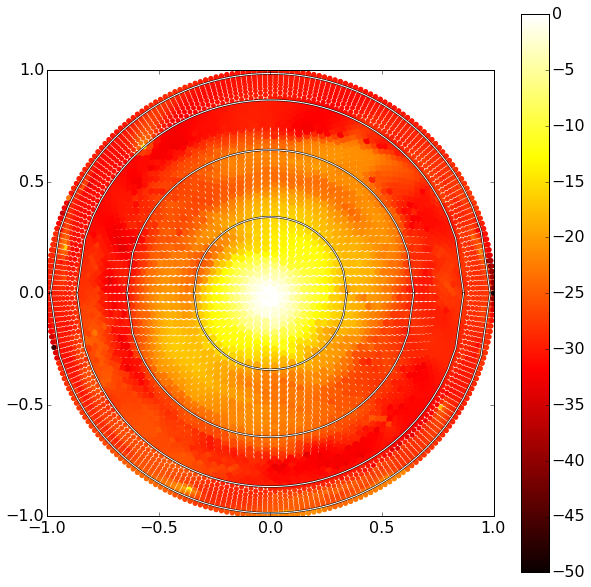
\includegraphics[width=3.5in]{measbeam_interp.png}
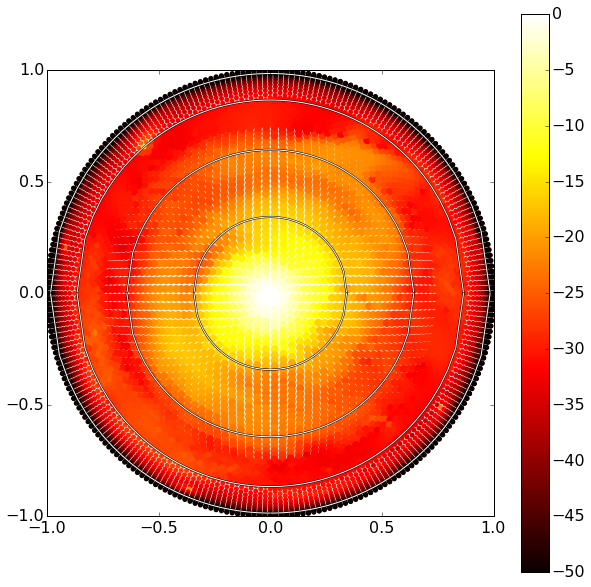
\includegraphics[width=3.5in]{measbeam_interp_expcutoff.png}
\caption{We construct full sky beams as required for Section \ref{sec:foregroundleakage} by starting from the nominal focus beam (top left), interpolating over unobserved cells at $\theta\lesssim60^\circ$ and extrapolating to the horizon (top right), and applying a gaussian cutoff starting at $\theta=60^\circ$ with $\sigma=2.5^\circ$ (bottom left). These last two beams span the space of likely horizon responses. Circles denote $\theta=20^\circ,40^\circ,60^\circ,80^\circ$.}
\label{fig:interpbeams}
\end{figure}

\begin{figure}[h]
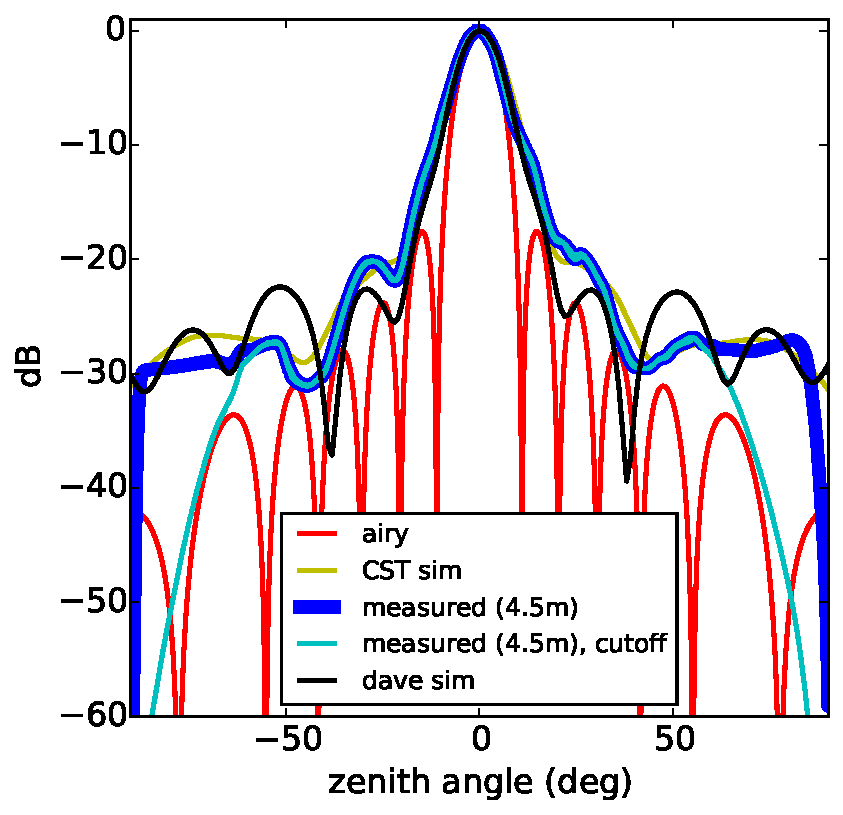
\includegraphics[width=3.5in]{ew_beams_slice.pdf}
\caption{We plot the interpolated/extrapolated measured nominal focus  beam itself (blue), and with the gaussian cutoff (cyan), along with various model beams to illustrate the varying horizon responses. }
\label{fig:interpbeamsslice}
\end{figure}

To illustrate the results of these smoothing operations we plot slices through the nominal focus dish beam along with the three model beams discussed in Sec. \ref{sec:dishmodels}. The H (E) plane slice of the main lobe is shown at the top (bottom). The plots in the left side zoom in on the main lobe, while those on the right show a zoomed out view of the entire sky pattern. 

\subsection{Collecting Area}

The collecting area of the antenna is related to the power pattern by the ratio of the beam gain to its beam-weighted solid angle as
\begin{equation}
	A=\frac{\lambda^2 B(0,0)}{\int B(\theta,\phi)d\Omega}
\end{equation}
We evaluate the collecting area for four of the beams discussed above and present the numbers in Table 1. We are unable to quantify the collecting area of the beam from Dave's simulation because it was run at too coarse an angular resolution. For the measured beams, we compute the collecting area using the interpolated/extrapolated beams with and without the gaussian cutoff at $\theta=60^\circ$.

 \begin{table}[h]
 \caption{ \label{table:collectingareatable}Collecting area (m$^2$) for modeled and measured dish beams at 137\,MHz. For measured beams, we calculate the collecting area after interpolation/extrapolation, also with the $60^\circ$ gaussian cutoff (in parentheses).}
\begin{tabular}{| l | l | l |}
\hline
  Airy & 155\,  \\
  CST sim & 67.0\,  \\
  \hline
  Measured, feed at 4\,m & 42.1 (44.3) \\
  Measured, feed at 4.5\,m & 68.5 (73.6) \\ 
  Measured, feed at 5\,m & 77.1 (82.6) \\
  Measured, feed at 5.3\,m & 93.0 (97.9)\\
  \hline
\end{tabular}
\end{table}

By definition, the Airy pattern has the largest collecting area equal to the dish cross section. The others model a realistic feed with a hanging screen (the skirt or ``kilt''), effectively tapering the dish response to radiation received from its fringes to mitigate cross-coupling and crosstalk between adjacent dishes. As expected, raising the height of the feed increases the illuminated area of the dish, and thus, its collecting area. As expected, the measured collecting area matches that of the CST model at the nominal focus height of 4.5\,m.

Why does the collecting area increase as the feed is raised over the nominal focus? There are two computing effects here: (1) the reflected radiation is less well focused above the feed, decreasing the response; and (2) the tapered feed sees a larger dish as it is raised, allowing more radiation to reach the dipole as opposed to reflecting off the skirt. These data suggest that the second effect wins. Of course the reason for the skirt is to taper the feed beam in order to mitigate cross-talk and cross-coupling between the dishes. A larger collecting area may not be worth it in exchange for exacerbating these concerns.

\section{Foreground Leakage and Residuals}
\label{sec:foregroundleakage}

We assess the level of foreground leakage into the EOR window due to beam shape, baseline length, and LST. In particular, we built on the study of \citet{nithya15} of the impact of beam shape and horizon response on foreground spectral structure and containment in the wedge.

We simulate delay spectra for several model and measured beams on different baseline lengths for different LSTs and baseline orientations. All these factors affect the level of emission horizon brightening in delay space, the ``pitchfork'' effect, and the level of foreground leakage. We assume a constant beam pattern over that band, with leakage due only to the finite bandwidth and choice of window function. Actual frequency structure imprinted onto the foregrounds by variation of the beam angular pattern or overall gain with frequency (Patra et al.)

We begin by simulating visibilities over a 20\,MHz bandwidth with  400\,kHz resolution centered on 137\,MHz on two different baselines for two model beams (airy, and CST sim) and two measured beams (measured nominal focus beam, and measured nominal focus beam with $60^\circ$ cutoff). We use the short and maximally redundant 14\,m baseline, most useful for delay spectrum analysis, as well as a longer 42\,m baseline, more useful for imaging analysis. From these frequency-sequenced visibilities we calculate the delay spectrum  \citep{perbaselinetechnique} using the Blackman-Harris window following \citet{nithya15}. This window reduces the noise equivalent bandwidth to 10\,MHz, corresponding to $\Delta z\sim0.5$, beyond which evolution of the cosmological signal become significant. Larger bandwidths, though, are useful for foreground estimation and delay-space deconvolution \citep{parsonsandbacker,paper32,paper64}. With this caveat, our simulated delay spectra show the worst case scenario, quantifying the level of foreground isolation without estimation and deconvolution.

Our sky model is comprised of a deep MWA point source survey within 20$^\circ$ of R.A.(J2000) $= 0^\text{h}\,0^\text{m}\,0^\text{s}$ and decl.(J2000) $= -30^\circ\,0'\,0''$ (Carroll et al., in prep.), the shallower but wider MWA commissioning point source survey\citep{MWACS}, the Culgoora catalog\citep{Slee1995}, and the Global Sky Model of Galactic radio emission \citep{gsm}. 

Figure \ref{fig:delayspec} shows the delay spectra at $0^\circ$ (top pair) and $60^\circ$ (bottom pair) LST for 14\,m (left pair) and 42\,m (right pair) EW baselines. For reference we plot a 1D model 21\,m power spectrum for $z\sim8$ from \citet{21cmfast}. Consider first the $0^\circ$ LST plots where the Galactic disk has nearly, but not completely set. The effect of horizon response is most visible on the longer 42\,m baseline where the measured beam (red) and CST model (yellow), both show significant brightening at the horizon delays (vertical black lines) due to roughly -30\,dB beam response near the horizon, as discussed by \citet{nithya15,nithya15}. In contrast, the airy model (black) and measured beam with cutoff (blue) show no significant brightening at the horizon, where they appear still to be dominated by the wings of the delay PSF from the emission closer to zero delay. 

We also plot (green dashed line) the delay spectrum after subtracting the visibilities computed with the $\theta\sim60^\circ$ cutoff measured beam from those using the full measured beam. This curve may be interpreted as the uncertainty in the ``pitchfork'' horizon brightening due to uncertainty in the beam horizon response, or equivalently as the delay spectrum residual foregrounds after subtracting foregrounds in the well modeled region of the sky. By construction, this subtraction leaves emission from the highest delay regions of the sky (near the horizon on opposite sides of the baseline), but also leaves some low delay emission on opposite sides of a line perpendicular to the baseline. However, this additional low delay emission near the horizon gets drowned out by that from near zenith where the beam is substantially stronger. 

On the shorter 14\,m baseline, the horizon brightening is smaller because there is roughly an order of magnitude more emission at zero delay, whose thereby stronger delay wings, which are also relatively wider compared to the narrower foreground wedge, cover up much of the edge brightening. At $60^\circ$ LST, effect of horizon response is much smaller as the Galactic disk is now entirely below the horizon. 

The level of leakage depends also on baseline orientation which sets which directions on the sky map to large delays. Figure \ref{fig:delayspec2} shows the delay spectra at $0^\circ$ LST on 14\,m NE (top pair) and SE (bottom pair) baselines. Both show increased edge brightening compared to the 14\,m EW baseline. \citet{nithya15} proposes to identify through modeling the baselines most susceptible to this edge brightening at any given time, and simply exclude them from the power spectrum analysis. 



\begin{figure*}[h]
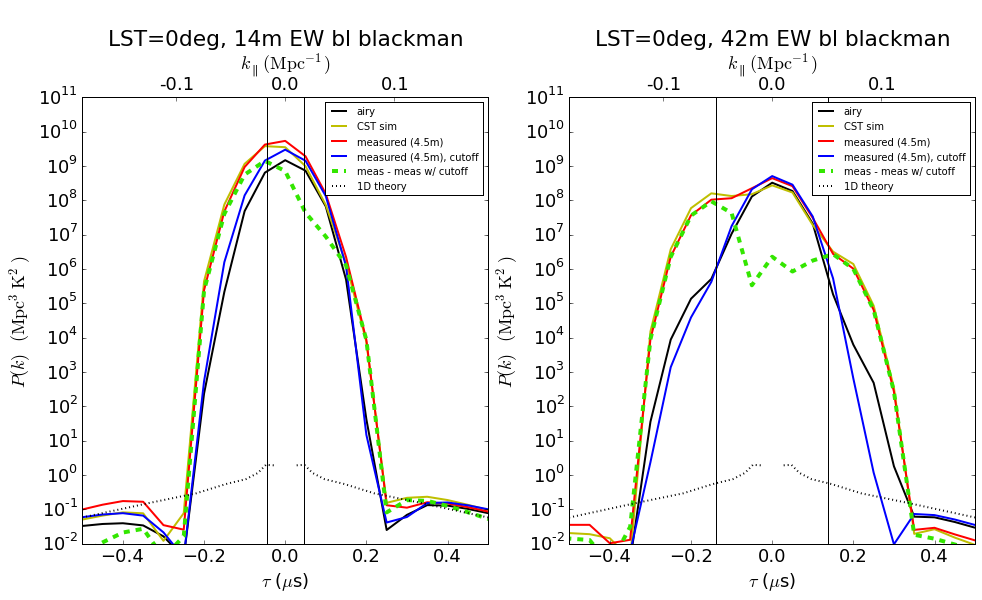
\includegraphics[width=6.7in]{LST0deg_14m_42m_EWbaselines_dish1_blackman.png}
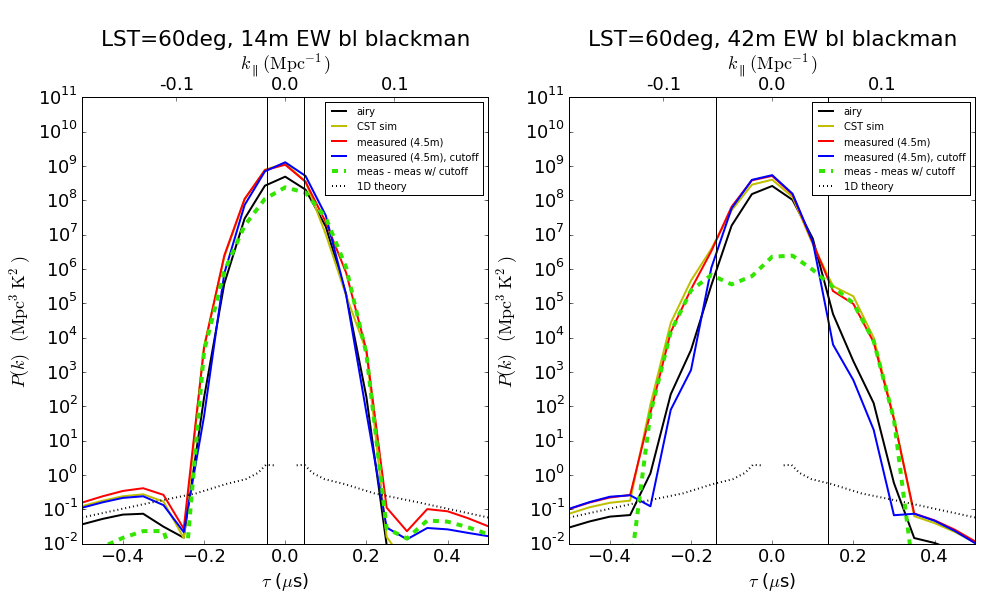
\includegraphics[width=6.7in]{LST60deg_14m_42m_EWbaselines_dish1_blackman.png}
\caption{Simulated delay spectra for the GSM and point sources at $0^\circ$ (top pair) and $60^\circ$ (bottom pair) LST for EW baselines of length 14\,m (left pair) and 42\,m (right pair). The beams are are assumed constant over frequency.}
\label{fig:delayspec}
\end{figure*}

\begin{figure*}[h]
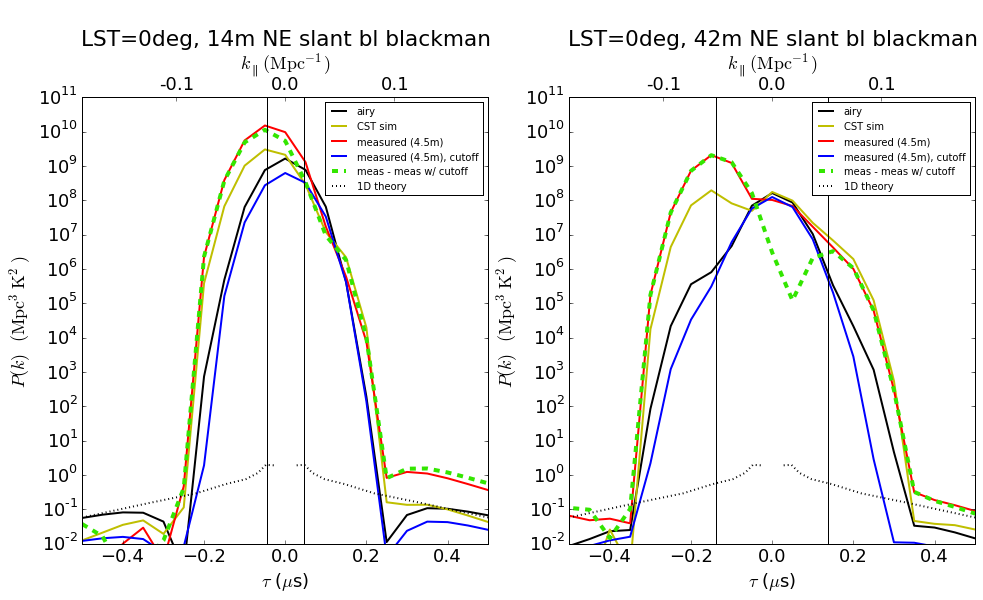
\includegraphics[width=6.7in]{LST0deg_14m_42m_NEslantbaselines_dish1_blackman.png}
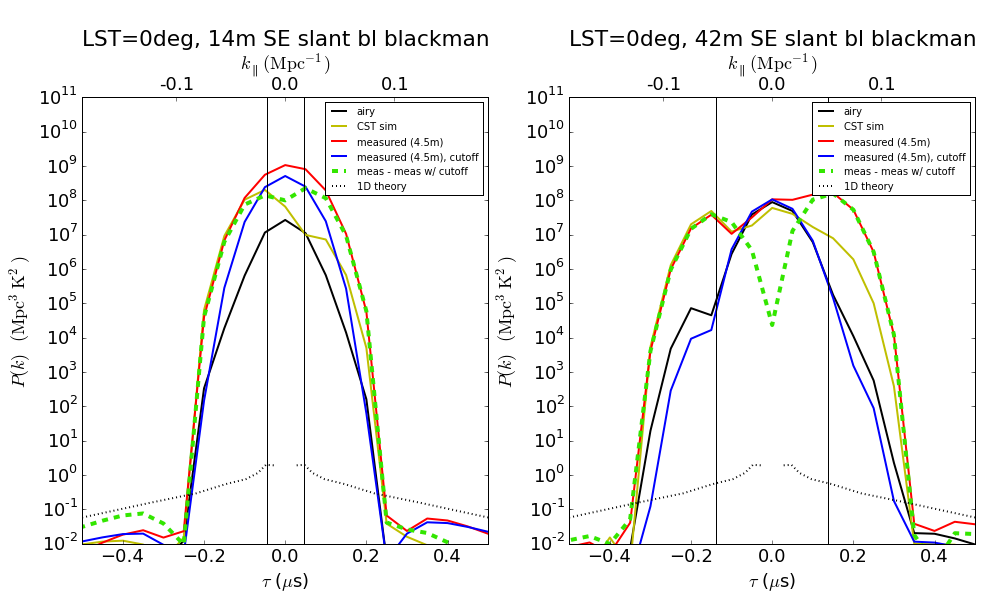
\includegraphics[width=6.7in]{LST0deg_14m_42m_SEslantbaselines_dish1_blackman.png}
\caption{Simulated delay spectra for the GSM and point sources at $0^\circ$ LST for NE (top pair) and SE (bottom pair) baselines of length 14\,m (left pair) and 42\,m (right pair). The beams are are assumed constant over frequency.}
\label{fig:delayspec2}
\end{figure*}





%\section{Discussion}

%As expected, the Airy patter has the largest collecting area

%the beam might be narrower simply because more dish is illuminated, but not necessarily a good thing, because we want more taper at the edge


%comment on how this expt is still a work in progress









%% The reference list follows the main body and any appendices.
%% Use LaTeX's thebibliography environment to mark up your reference list.
%% Note \begin{thebibliography} is followed by an empty set of
%% curly braces.  If you forget this, LaTeX will generate the error
%% "Perhaps a missing \item?".
%%
%% thebibliography produces citations in the text using \bibitem-\cite
%% cross-referencing. Each reference is preceded by a
%% \bibitem command that defines in curly braces the KEY that corresponds
%% to the KEY in the \cite commands (see the first section above).
%% Make sure that you provide a unique KEY for every \bibitem or else the
%% paper will not LaTeX. The square brackets should contain
%% the citation text that LaTeX will insert in
%% place of the \cite commands.

%% We have used macros to produce journal name abbreviations.
%% AASTeX provides a number of these for the more frequently-cited journals.
%% See the Author Guide for a list of them.

%% Note that the style of the \bibitem labels (in []) is slightly
%% different from previous examples.  The natbib system solves a host
%% of citation expression problems, but it is necessary to clearly
%% delimit the year from the author name used in the citation.
%% See the natbib documentation for more details and options.

\bibliography{DishBeamMeasurementsMemo}


\end{document}
-